\documentclass[a4paper, % A4
	parskip, % Absätze durch Abstand statt Einrückung gekennzeichnet
	%draft, % überlange Zeilen werden nicht%markiert
	ngerman] % english, hyphenation etc.
	{scrreprt} % Report (KOMA-Script)

\usepackage{fontspec}

\usepackage[babel]{microtype} % Automatische Grauwertverbesserung
\usepackage[ngerman]{babel} % warning that option english is not loaded yet
    % when not declaring [USenglish] even though documentclass sets it globally
\usepackage{IEEEtrantools} % bibliography, quoting (\cite)

\usepackage{graphicx} % include images (\includegrafics)
\usepackage[section]{placeins} % place floating objects before a \FloatBarrier

\usepackage{framed} % frame paragraphs (\begin{framed})
\usepackage{geometry} % change margin for title page (\newgeometry,
	% \resetgeometry)
\usepackage{setspace} % change line spacing (\onehalfspacing)
\usepackage{pdflscape} % pages in landscape (\begin{landscape})
\usepackage{multicol} % multiple columns for a sector (\begin{multicols})

\usepackage{booktabs} % Professional looking tables (\toprule,% \midrule,
	% \bottomrule)
\usepackage{threeparttable} % table with notes (\tnote, \begin{tablenotes})
\usepackage{longtable}

% Redefine space before and after chapter title
\renewcommand*{\chapterheadstartvskip}{\vspace*{12pt}}
\renewcommand*{\chapterheadendvskip}{\vspace*{12pt}}

\usepackage[printonlyused, % show only used acronyms
		% withpage, % show pagenumber of first usage
	] % longform in footnote (instead of shortform)
	{acronym} % abbreviations  (\ac, \acs,\acl)
		% \begin{acronym})
		
\usepackage{pdfpages} % include PDFs (\includepdf)
\usepackage{float} % own floating objects (\newfloat, \floatname)

\usepackage{hyperref} % linking to refs and URLs (\ref, \url, \autoref,
% \nameref)
%rename the output for an \autoref{chap:XXX} from lowercase chapter to Chapter
% and also for Section and Subsection
\addto\extrasUS{%
  \renewcommand{\chapterautorefname}{Chapter}% 
}
\addto\extrasUSenglish{%
  \renewcommand{\sectionautorefname}{Section}% 
}
\addto\extrasUSenglish{%
  \renewcommand{\subsectionautorefname}{Subsection}% 
}

\setcounter{secnumdepth}{3}

% global formatting
\onehalfspacing % 1.5x line spacing

\usepackage{color}

%Package for syntax highlighting (needs pygments installed): https://tex.stackexchange.com/a/256796
\usepackage{caption}
\usepackage[newfloat]{minted}
\captionsetup[listing]{}
\captionsetup{labelfont=bf}

% Default options for python code
\setminted[python]{linenos, frame=leftline, numbersep=8pt, framesep=8pt, tabsize=4}

% bigger line numbers for code blocks
\renewcommand{\theFancyVerbLine}{\sffamily {\small \oldstylenums{\arabic{FancyVerbLine}}}}

\newcommand{\code}[1]
	{\texttt{#1}}
\newcommand{\command}[1]
    {\textit{#1}}
\newcommand{\filepath}[1]
	{\texttt{#1}}
\newcommand*{\fullref}[1]
    {\hyperref[{#1}]{\autoref*{#1} \nameref*{#1} on page \pageref*{#1}}}
\newcommand{\linenumber}[1]
    {\textit{#1}}
\newcommand{\productname}[1]
	{\textit{#1}}
\newcommand{\tbd}[1]
    {{\color{red}<tbd> #1}}
\newfloat{listingfloat}{htb}{qcl}[chapter]
\floatname{listingfloat}{Listing}

% definiton of frequenlty used standard texts.
% Usage in text: \authors{} -> Jonas Matter, Robin Suter

\newcommand{\advisor}
	{Prof. Stefan Keller}
\newcommand{\authors}
	{Jonas Matter, Robin Suter}
\newcommand{\place}
	{HSR---University of Applied Sciences Rapperswil \\ Institute for
	Software}
\newcommand{\timeperiod}
	{Herbstsemester 2017}
\newcommand{\titel}
	{PlazaRoute}
\newcommand{\work}
	{Studienarbeit}

\loadglsentries{appendix/glossary}
\makeglossaries

\begin{document}
\setromanfont[BoldFont={Gentium Basic Bold},ItalicFont={Gentium Basic Italic}]{Gentium Basic}

% Following the template unter www.hsr.ch > HSR-intern > Bachelor-Studiengänge
% > Informatik > allgemeine Infos Diplom-, Bachelor- und Studienarbeiten.

\newgeometry{left=2.25cm, right=2.25cm, top=2.25cm, bottom=2.25cm} % new
% margins

\begin{titlepage}

\begin{center}
\begin{minipage}[t]{0.45\textwidth}
    
\includegraphics[width=\textwidth]{start/img/hsrLogo}
\end{minipage}
\hspace{\fill} % horizontal space
\begin{minipage}[t]{0.45\textwidth}
    \vspace{-2.56cm}
    
\includegraphics[width=\textwidth]{start/img/ifsLogo}
\end{minipage}

\end{center}

\vspace{15ex} % vertical space
\Huge 
\textbf{\titel}

\vspace{3ex}
\textbf{\work}

\vspace{1ex}
\LARGE 
\place

\vspace{5ex}
\timeperiod

\vspace{11ex}
\begin{tabular}{ll} % Table
	Autoren:        & \authors    \\
	Betreuer:        & \advisor    \\
\end{tabular}

\end{titlepage}

\restoregeometry % reset page margins


% Der Abstract richtet sich an den Spezialisten auf dem entsprechenden Gebiet
% und beschreibt daher in erster Linie die (neuen, eigenen) Ergebnisse und
% Resultate der Arbeit. Es umfasst nie mehr als eine Seite, typisch sogar nur
% etwa 200 Worte (etwa 20 Zeilen). Es sind keine Bilder zu verwenden.

\chapter*{Abstract}\addcontentsline{toc}{chapter}{Abstract}

Die heutig gängigen Routing-Engines sind für den motorisierten Individualverkehr optimiert. Bei diesem halten sich die Verkehrsteilnehmer an vorgegebene Regeln und Strecken. Fussgänger allerdings optimieren intuitiv ihre Route, so wählen sie zum Beispiel über eine öffentliche Fläche den möglichst kürzesten Weg zum Ziel. Bestehende Routing-Engines navigieren entlang der Kante des Platzes, anstatt ihn direkt zu überqueren.

Es werden bestehende Algorithmen zur Traversierung von offenen Fussgänger-Flächen evaluiert, analysiert und optimiert. Mit einer Vorverarbeitung von OpenStreetMap-Daten wird gezeigt, wie eine Routing-Engine ein natürliches Fussgänger-Routing durch offene Flächen unterstützen kann.

Als praktisches Beispiel wird mit Hilfe des Services von search.ch ein Prototyp für ein multimodales Routing mit öffentlichen Verkehrsmitteln erarbeitet. Mit einem eigens entwickelten Plugin für QGIS können die optimierten Routen visualisiert werden.

Durch die Vorverarbeitung von OpenStreetMap-Daten ist die Grundlage für ein natürliches Fussgänger-Routing geschaffen, auf welche gängige Routing-Engines aufsetzen können. Die eingesetzen Algorithmen zeigen deutlich bessere Ergebnisse als die bestehenden Implementationen in den Routing-Engines.

Mit dem entwickelten Prototypen und einem zugehörigen QGIS-Plugin können Benutzer mit einem beliebigen Start- und Endpunkt ein ÖV-Routing mit optimiertem Verhalten bei Fussgänger-Routen durchführen.

\cleardoublepage

Today's most notable open source routing engines are optimized for motorized traffic, but show deficiencies when it comes to pedestrian routing. With open spaces, routers usually navigate along the edges of the polygon, whereas pedestrians would naturally take shortcuts through the open space while avoiding any obstacles.
Past research has shown multiple approaches to this problem. In this thesis, some of these are approaches are compared and analysed.

With publicly available geographic data from OpenStreetMap and the help of these algorithms, a proof-of-concept implementation is provided to prepare geographic data for an existing routing engine, with the aim of enhancing it with the capabilities to provide a natural behavior in pedestrian routing. The preparation step is optimized with shortest-path algorithms to keep the additional data volume as low as possible.

Furthermore, the optimized routing is used in combination with an existing service for public transport routing in Switzerland, providing a practical application with multimodal transportation. With a newly-developed plugin for QGIS, users are able to visualize the optimized routes.

The implementation of two different approaches --- visibility graph and SpiderWeb graph --- shows a clear improvement on routes for pedestrian navigation, compared to the methods that are used in current routing engines. In the future, this implementation could serve as a reference to integrate these approaches directly into routing engines.
% Das Management Summary richtet sich in der Praxis an die "Chefs des Chefs", d.
% h. an die Vorgesetzten des Auftraggebers (diese sind in der Regel keine
% Fachspezialisten).
% Die Sprache soll knapp, klar und stark untergliedert sein.
% Zu verwenden ist folgenden Gliederung:
% - Ausgangslage - Vorgehen, Technologien - Ergebnisse - Ausblick (optional)

\chapter*{Management Summary}\addcontentsline{toc}{chapter}{Management Summary}

% TODO: 3 - 4 Seiten, 2 Bilder mit Outlook

% hier eine kurze Einleitung

\textbf{Ausgangslage}

\textbf{Vorgehen und Technologien}

\textbf{Ergebnisse}

\textbf{Ausblick}

\addcontentsline{toc}{chapter}{Inhaltsverzeichnis}
\tableofcontents

\addcontentsline{toc}{chapter}{Aufgabenstellung}
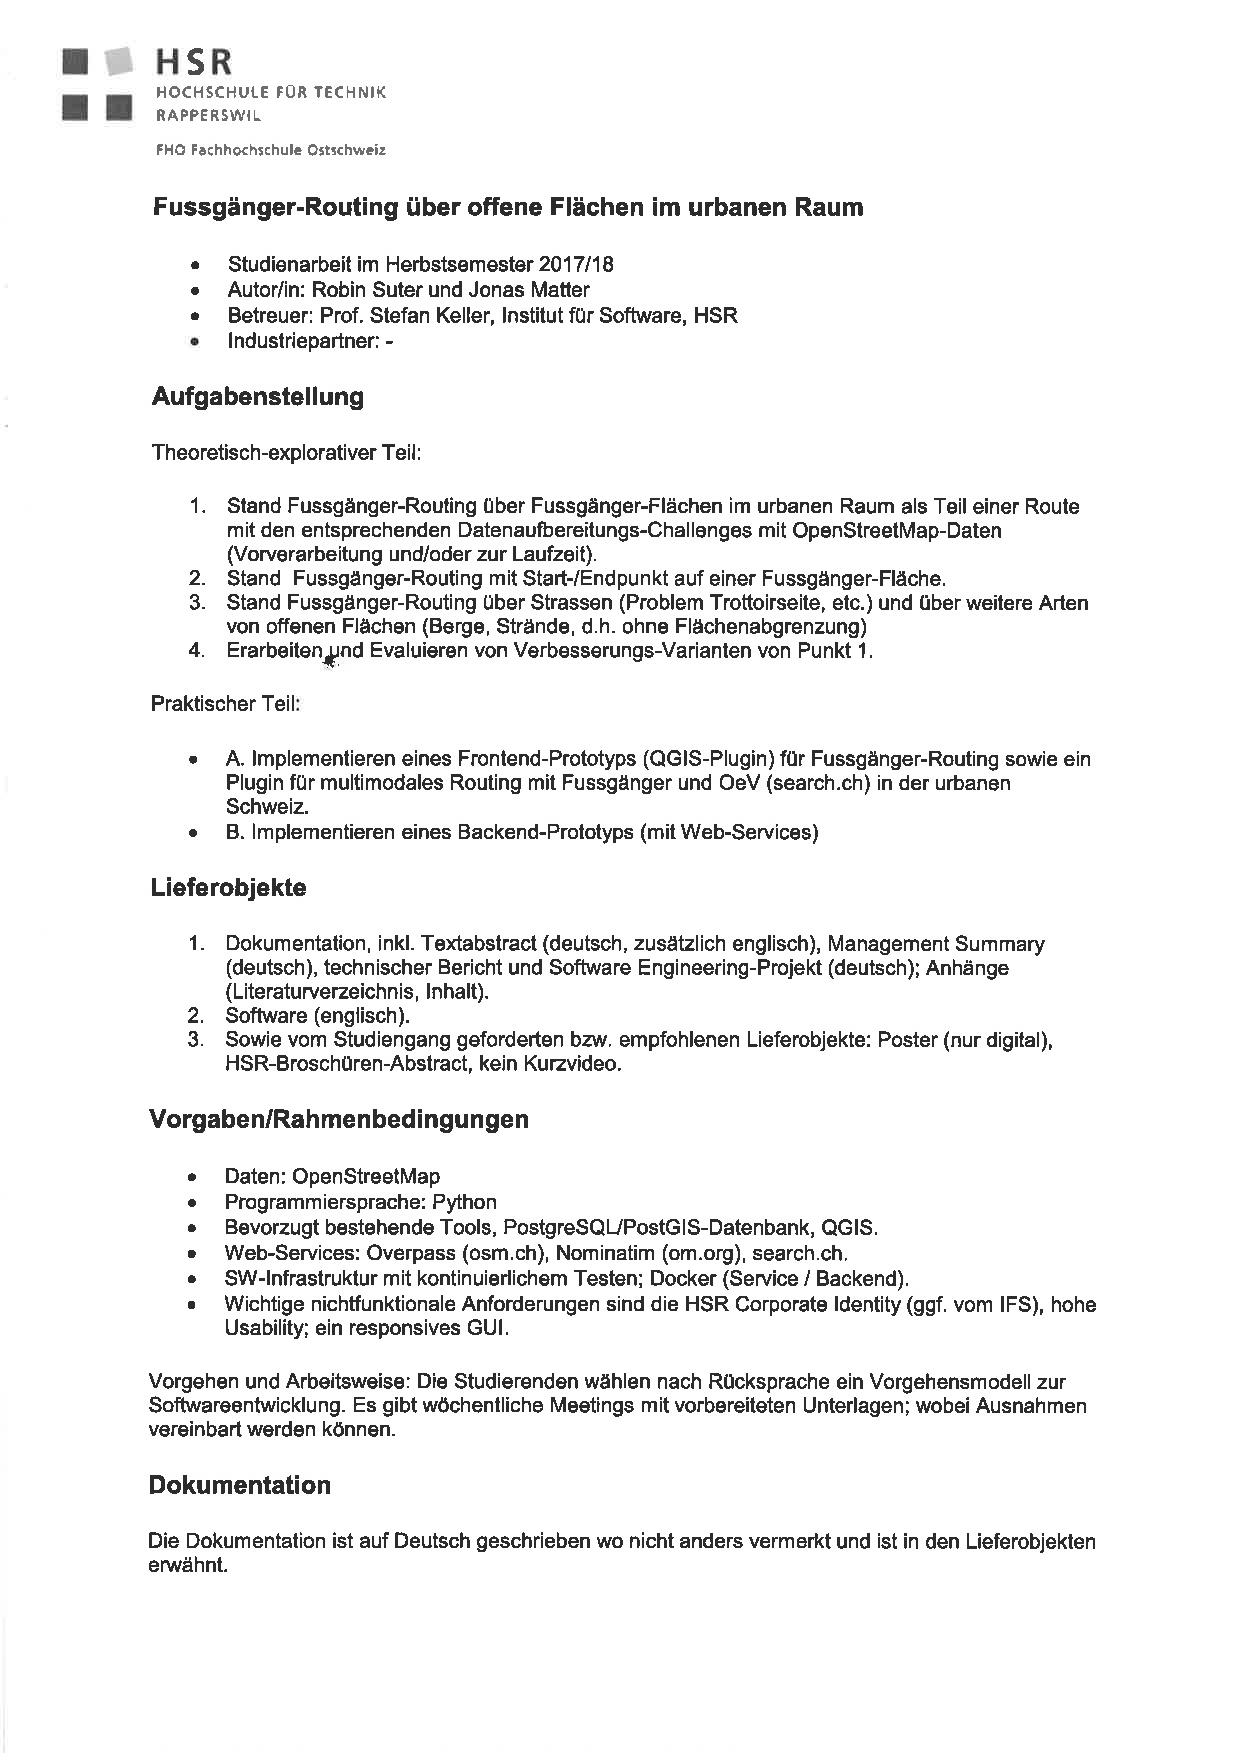
\includepdf[pages=-]{additionals/assignment.pdf}


% Summary index document for ...

\chapter{Technischer Bericht}
\label{chap:Technischer Bericht}

\section{Einführung}
\label{Einführung}
Diese Arbeit befasst sich grundlegend mit dem Fussgänger-Routing und Auffinden der nächsten ÖV-Haltestelle, welche einem an ein weiter gelegenes Ziel führen kann. Ziel ist es, von einem gegebenen Punkt die nächste ÖV-Haltestelle, welche zu Fuss erreichbar ist, zu finden. Im folgenden ist die Problemstellung erläutert und es wird eine Abgrenzung gemacht, was Teil dieser Arbeit ist.

\subsection{Problemstellung und Vision}
\label{Problemstellung und Vision}
Die heutig gängigen Routing-Engines können effizient über Kanten und Knoten routen, um so den schnellstmöglichen Weg finden zu können. Diese wurden stetig für Autofahrer optimiert, da sich diese unter anderem an vorgegebene Regeln halten. Beim nicht-motorisierten Individualverkehr (Fussgänger, Rollstuhlfahrer, Radfahrer, etc.)  ist das nicht immer der Fall. In den folgenden Unterkapiteln werden einige Probleme erläutert, welche immer noch Praxis für den nicht-motorisierten Individualverkehr sind.

\subsubsection{Routing über offene Flächen}
\label{problem:Routing über offene Flächen}
% TODO Verweis auf GraphHopper?
Wie man an in der Abbildung \ref{fig:helvetiaplatz_graphhopper} gut sieht, routet die Routing-Engine GraphHopper den Kanten nach um den Platz herum. Dies ist ein natürliches Verhalten für den motorisierten Individualverkehr. Ein Fussgänger hingegen nimmt den direkten Weg über den Platz. Oft handelt es sich nicht nur um einen leeren Platz, sondern es sind darauf Hindernisse wie Brunnen, Kunstwerke, WCs, etc. stationiert, um welche auf eine natürliche Weise geroutet werden muss. Eine Route, welche direkt auf das Hindernis zusteuert, um dieses dann zu umlaufen, ist zwar ein Fortschritt zur aktuellen Lösung, entspricht aber kaum einem normalen Fussgänger-Verhalten. 

\begin{figure}[ht]
	\centering
	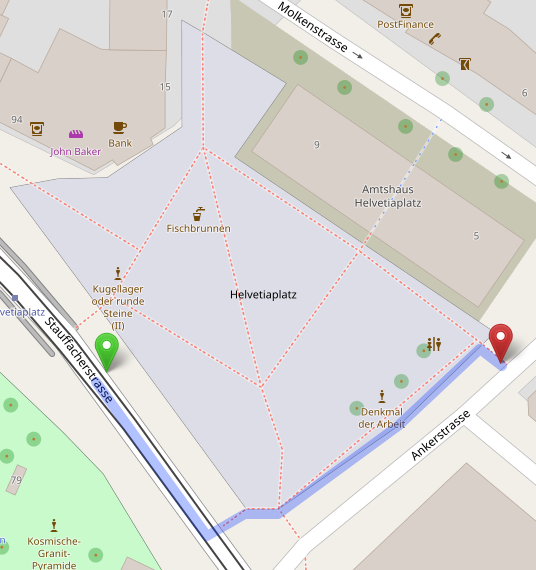
\includegraphics[width=0.5\linewidth]{technicalreport/img/helvetiaplatz_graphhopper}
	\caption[Fussgänger-Routing]{Fussgänger-Routing mit GraphHopper über den Helvetiaplatz, Zürich, Schweiz; Screenshot von openstreetmap.org aufgenommen am 08.10.2017}
	\label{fig:helvetiaplatz_graphhopper}
\end{figure}

\subsubsection{eingezeichnete Fussgängerrouten über offene Flächen}
\label{problem:eingezeichnete Fussgängerrouten über offene Flächen}
Wenn man die gleiche Abbildung \ref{fig:helvetiaplatz_graphhopper} nochmals betrachtet, sieht man, dass Mapper bereits einige Fussgängerwege auf dem Platz eingezeichnet haben, um dem Routing-Problem über offene Fläche entgegen zu steuern. Dies kann in einigen Situationen wie dem Helvetiaplatz kontraproduktiv, aber in anderen wieder von Vorteil sein. Betrachtet man beispielsweise den Central Park in New York in Abbildung \ref{fig:central_park} macht es Sinn, dass das Routing den vorgegeben Wegen folgt. Eine Wiese gilt als offene Fläche, eignet sich aber nicht immer als vorteilhafter Bewegungsuntergrund. Man muss abklären, in welchen Situation man sich auf vorhandene Wege über offene Flächen verlassen kann und wann sie zu ignorieren sind. Es gilt zu prüfen, ob diese Abgrenzung mit den gegebenen Informationen überhaupt möglich ist.

\begin{figure}[ht]
\centering
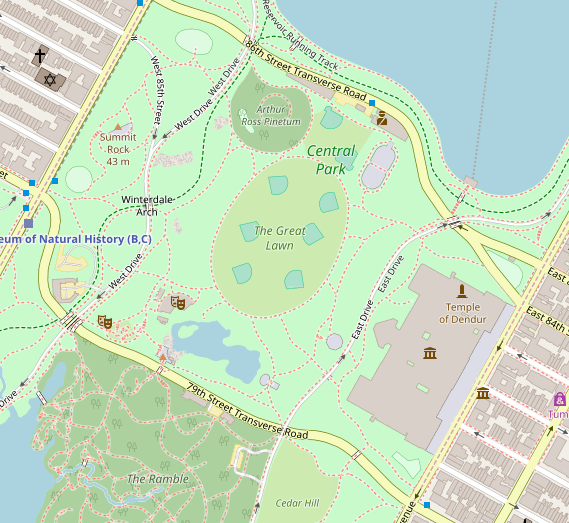
\includegraphics[width=0.5\linewidth]{technicalreport/img/central_park}
\caption[eingezeichnete Fussgänger-Routen]{Eingezeichnete Fussgänger-Routen auf dem Central Park, New York City, USA; Screenshot von openstreetmap.org aufgenommen am 08.10.2017}
\label{fig:central_park}
\end{figure}

\subsubsection{topologisch nicht verbundene Wege}
\label{problem:topologisch nicht verbundene Wege}

\begin{figure}[ht]
\centering
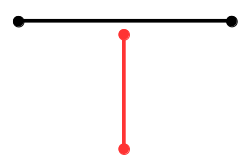
\includegraphics[width=0.5\linewidth]{technicalreport/img/topologisch_nicht_verbundener_graph}
\caption[topologisch nicht verbundener Graph]{topologisch nicht verbundener Graph}
\label{fig:topologisch_nicht_verbundener_graph}
\end{figure}

In Abbildung \ref{fig:topologisch_nicht_verbundener_graph} ist ein topologisch nicht verbundener Graph zu sehen. In \ac{OSM} kann es vorkommen, dass solche Wege auf eine offene Fläche treffen, mit dieser aber nicht topologisch verbunden sind. Eine Routing-Engine muss in der Lage sein, dies zu erkennen und aufzuräumen, so dass vom auftreffenden Weg über die offene Fläche geroutet werden kann.

\subsubsection{Routing über über weitere Arten von offenen Flächen (Berge, Strände)}
\label{problem:Routing über über weitere Arten von offenen Flächen (Berge, Strände)}
Berge und Strände sind bekanntermassen schwieriger zu überqueren als normale Plätze. Sei dies aufgrund der zurückzulegenden Höhendifferenz oder die Unterlage, welche das Fortbewegen mühsamer macht. Zusätzlich zum Problem \ref{problem:Routing über offene Flächen} kommt hier dazu, dass Umlaufen dieser offenen Flächen (Berge, Strände) effizienter sein kann als das Überqueren.

\subsubsection{Start-/Endpunkt auf der Fläche}
\label{problem:Start-/Endpunkt auf der Fläche}
Beginnt das Routing oder ist der Zielort auf einer Fläche, so ziehen die aktuellen Routing-Engines, falls keine Wege wie in \ref{problem:eingezeichnete Fussgängerrouten über offene Flächen} beschrieben eingezeichnet sind, eine rechtwinklige Linie zur nächsten Kante der Fläche und routen von dort weiter. Dies ist gut auf dem Sechseläutenplatz in Abbildung \ref{fig:start_endpoint_on_area} sichtbar. Falls bereits Wege auf der Fläche eingezeichnet sind, wird über diese geroutet.

\begin{figure}[ht]
    \centering
    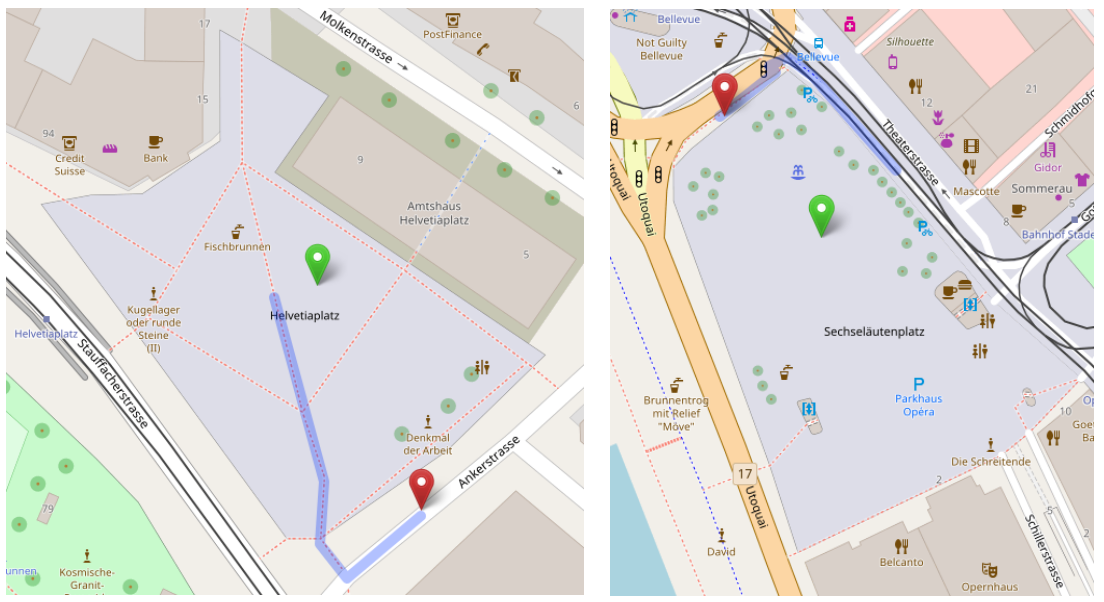
\includegraphics[width=1\linewidth]{technicalreport/img/start_endpoint_on_area}
    \caption[Fussgänger-Routing mit Startpunkt auf der Fläche]{Fussgänger-Routing mit GraphHopper über den Helvetiaplatz (links) und Sechseläutenplatz (rechts), Zürich, Schweiz mit Startpunkt auf der Fläche; Screenshot von openstreetmap.org aufgenommen am 14.10.2017}
    \label{fig:start_endpoint_on_area}
\end{figure}

\subsubsection{Routing bei zwei benachbarten Flächen}
\label{problem:Routing bei zwei benachbarten Flächen}
Es kann vorkommen, dass zwei Flächen unmittelbar nebeneinander liegen. Dies ist beim Bundesplatz in Bern, Schweiz der Fall, welcher direkt an den Bärenplatz grenzt. Dies ist in Abbildung \ref{fig:bundesplatz_baerenplatz} sichtbar. Das erschwert das Routing über Flächen, da nicht direkt Entry-Points eines Polygons genutzt werden können.

\begin{figure}[ht]
\centering
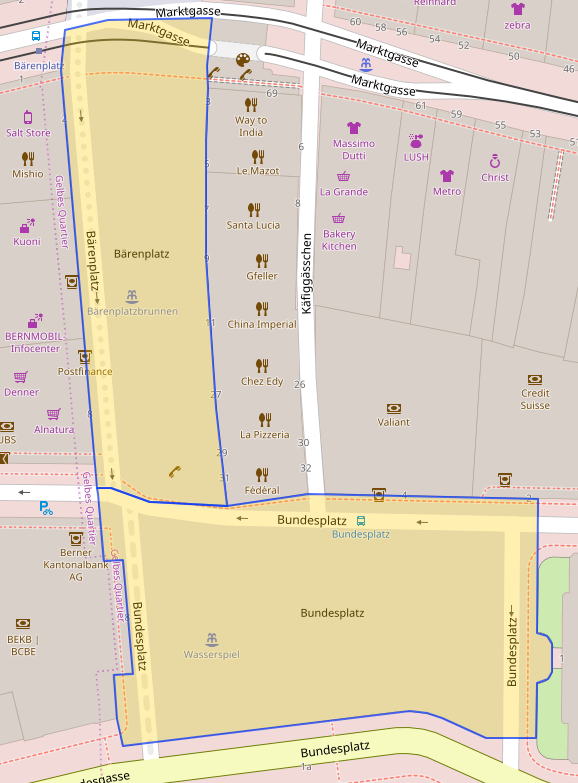
\includegraphics[width=0.5\linewidth]{technicalreport/img/bundesplatz_baerenplatz}
\caption[Zwei benachbarte Flächen]{Zwei benachbarte Flächen (Bundesplatz, Bärenplatz) in Bern, Schweiz; Screenshot von overpass-turbo.eu aufgenommen am 18.10.2017}
\label{fig:bundesplatz_baerenplatz}
\end{figure}
	
\subsection{Ziele und Unterziele}
\label{Ziele und Unterziele}

\subsubsection{Routing über offene Flächen}
\label{target:Routing über offene Flächen}
Das Problem wie in \ref{problem:Routing über offene Flächen} beschrieben wurde bereits in einigen Arbeiten aufgegriffen \cite{graser_visibility_graph}, \cite{dzafic_spider_web_graph}. Diese beiden Ansätze (Visibility-Graph und SpiderWeb-Graph) werden analysiert, Tests in QGIS implementiert und getestet. Ziel ist es, die optimale Variante zu eruieren, um über offene Flächen den schnellstmöglichen Weg zu finden.

\subsubsection{Routing-Engine evaluieren}
\label{target:Routing-Enginge evaluieren}
Die zahlreichen Routing-Engines sollen analysiert und festgehalten werden, welche sich für den Hauptzweck dieser Arbeit am besten eignet. Zusätzlich wird geprüft, wie die Datenvorverarbeitung (Einzeichnen der Routen für Routing über offene Flächen) in die bestehenden Routing-Engines eingehängt werden kann.

\subsubsection{eingezeichnete Fussgängerrouten über offene Flächen}
\label{target:eingezeichnete Fussgängerrouten über offene Flächen}
Es soll eruiert werden, ob für den Platz die eingezeichneten Fussgängerrouten ignoriert werden können oder ob man an diese gebunden ist, wie man in Abbildung \ref{fig:central_park} sieht.

\subsubsection{topologisch nicht verbundene Wege}
\label{target:topologisch nicht verbundene Wege}
Dieses Problem ist der Vollständigkeit halber aufgeführt, wird in dieser Arbeit aber nicht weiter verfolgt.
%TODO bereits Teil der Routing-Engines

\subsubsection{Routing über über weitere Arten von offenen Flächen (Berge, Strände)}
\label{target:Routing über über weitere Arten von offenen Flächen (Berge, Strände)}
Im Kontext dieser Arbeit wird kurz ein theoretischer Ansatz aufgezeigt, wie man mit einem kostenbasierten Graph den Eigenschaften diesen Unterflächen gerecht werden könnte.

\subsubsection{Start-/Endpunkt auf der Fläche}
\label{target:Start-/Endpunkt auf der Fläche}
Der Start des Fussgänger-Routing ist von überall möglich. Somit soll es möglich sein, dass das Routing auf einer Fläche beginnen kann und man nicht wie in \ref{problem:Start-/Endpunkt auf der Fläche} beschrieben, zur nächstgelegenen Polygonkanten geroutet wird. Es soll geklärt werden, ob die Vorverarbeitung der Flächen, wie es in \ref{target:Routing über offene Flächen} vorgesehen ist, ausreicht, oder ob zu einem späteren Zeitpunkt ein Echtzeit-Verarbeitung der Fläche vom aktuellen Standort aus in Betracht gezogen werden muss.

\subsubsection{Routing bei zwei benachbarten Flächen}
\label{target:Routing bei zwei benachbarten Flächen}
Dieses Problem ist der Vollständigkeit halber aufgeführt, wird in dieser Arbeit aber nicht weiter verfolgt.

\subsubsection{nächste ÖV-Haltestellen finden}
\label{target:nächste ÖV-Haltestellen finden}
Der Fokus der Arbeit liegt auf dem Finden und Erreichen der nächsten ÖV-Haltestelle, welche einem ans gewünschte Ziel führt. So soll eruiert werden, wie von einem bestehenden Startpunkt aus die nächsten ÖV-Haltestellen identifiziert werden, um diese an search.ch für das weitere Routing zu übergeben.

\subsubsection{Prototyp}
\label{target:Prototyp}

% TODO was kommt in Prototyp, wie sieht er aus
TODO

\subsubsection{Deliverables}
\label{target:Deliverables}

% TODO was wird konkret abgeliefert?
TODO
	
\subsection{Rahmenbedingungen, Umfeld, Definitionen, Abgrenzungen}
\label{Rahmenbedingungen, Umfeld, Definitionen, Abgrenzungen}
Grundsätzlich befasst sich die Arbeit mit Flächen im urbanen Raum. Berge, Strände und Felder werden bewusst ausgeklammert, um nicht den Rahmen der Arbeit zu sprengen.

% TODO muss man hier noch Python, QGIS, search.ch erwähnen?

\subsection{Vorgehen und Aufbau der Arbeit}
\label{Vorgehen und Aufbau der Arbeit}
Die Studienarbeit nimmt sich zu erst dem Problem des Fussgänger-Routing über Flächen im urbanen Raum an. Es wird geklärt, wie momentan die Thematik gehandhabt wird und welche Vorarbeiten und Lösungen in diesem Bereich existieren. Bestehende Lösungsvorschläge werden mit der Hilfe von QGIS in Python implementiert, um so die bestmögliche Variante zu eruieren. Das gleiche Vorgehen wird für das Fussgänger-Routing über Strassen gewählt. Sobald die bestmöglichen Lösungsvarianten identifiziert sind, muss geklärt werden, wie die Vorverarbeitung der Daten (beispielsweise, das Einzeichnen von möglichen Routen über Flächen) an eine bestehende Routing-Engine übergeben werden kann. Damit dies möglich ist, ist zu prüfen, welche Engine die Anforderungen bestmöglich abdecken.

In einem weiteren Schritt soll ermittelt werden, wie die nächsten ÖV-Haltestellen eruiert werden können, um diese Punkte an die API von search.ch übergeben zu können. Aufgabe von search.ch ist es, für n Startpunkte die ÖV-Route zu genieren. So ist es möglich, denn schnellstmöglichen Weg für eine Route in Kombination von Fussweg und öffentlichem Weg zu ermitteln.

Die vorhin aufgeführten Aspekte werden im Kapitel \ref{chap:Technischer Bericht} behandelt.

In einem zweiten Teil werden die im Teil 1 erarbeiteten Artefakte zusammengeführt. Es wird in QGIS ein Prototyp implementiert. Die Ergebnisse werden im Kapitel \ref{chap:SW-Projektdokumentation} beschrieben.

% TODO wie sieht Prototyp genau aus


% TODO Grafik mit Epics und einigen Unterpunkten was dazu gehört

\subsection{Grundlagen und Begriffe}
\label{Grundlagen und Begriffe}

Im folgenden werden einige theoretische Grundlagen und Begriffe eingeführt, welche im Laufe des Dokuments auftauchen werden.

% TODO was muss alles noch eingeführt werden?


\subsubsection{Fläche}
\label{Fläche}

Als Fläche werden für diesen Zweck Plätze, Wiesen, etc. verstanden, die von Fussgänger frei begehbar sind. Flächen sind in \ac{OSM} keine eigenständige Datenelemente. Es handelt sich dabei um Polygone (sprich geschlossene Linien) oder Multipolygone (siehe \ref{Multipolygon}), welche in \ac{OSM} mit den Attributen \textit{landuse=*} oder mit \textit{highway=footway} und \textit{area=yes} versehen sind. Fehlt \textit{area=yes} wird die geschlossene Linie als Rundweg interpretiert, über welche nicht geroutet werden soll. \cite{osm_wiki_area}
% TODO: Wie genau filtern wir nach Flächen? Area=yes UND highway=pedestrian?

\subsubsection{nicht-motorisierter Individualverkehr}
\label{nicht-motorisierter Individualverkehr}

Zum nicht-motorisierten Individualverkehr gehören unter anderem Fussgänger, Rollstuhlfahrer und Radfahrer.

Zur besseren Lesbarkeit und der Einfachheit halber wird in der Arbeit nur noch von Fussgänger gesprochen.

\subsubsection{Multipolygon}
\label{Multipolygon}

Multipolygone in \ac{OSM} sind ein oder mehrere Polygone, die jeweils einen geschlossenen Pfad beschreiben. Jedes Polygon kann entweder als einen äusseren oder inneren Ring dienen. So kann ein innerer Ring eine Teilfläche eines äusseren Rings ausschneiden. Polygone in einem Multipolygon können auch disjunkt sein. \cite{osm_wiki_multipolygon}

\begin{figure}[th]
\centering
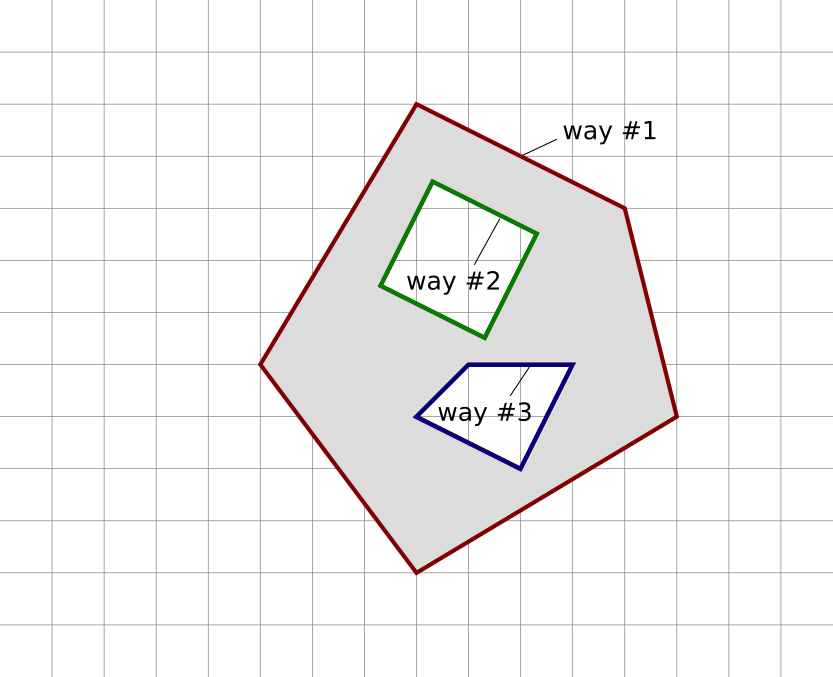
\includegraphics[width=0.5\linewidth]{technicalreport/img/multipolygon_osm_example.png}
\caption[Multipolygon OSM Example]{Beispiel eines Multipolygons in \ac{OSM} mit einem äusseren und zwei inneren Ringen. \cite{osm_wiki_multipolygon}}
\label{fig:multipolygon_osm_example}
\end{figure}

In GIS hingegen ist ein Multipolygon definiert als mehrere sich nicht überschneidende Polygone. Jedes Polygon wird durch ein oder mehrere geschlossene Pfade beschrieben. Dabei ist der erste Pfad der äussere Rand, alle weiteren Pfade beschreiben innere Ringe. \cite{opengis_simple_features}

\subsubsection{Hindernisse auf Flächen}
\label{Hindernisse in Flächen}

TODO % wie sieht Datenstruktur aus


\subsubsection{Shortest Path}
\label{Shortest Path}

TODO


\section{Stand der Technik}
\label{sec:Stand der Technik}

In \ac{OSM} gibt es mehrere Arten, wie Mapper mit Flächen umgehen. So wirken einige Mapper dem Fussgängerrouting-Problem über Flächen mit zusätzlichen eingezeichneten Wegen entgegen oder die Fläche ist ganz befreit von Wegen.

In Abbildung \ref{fig:helvetiaplatz_comparison} und Abbildung \ref{fig:sechselaeutenplatz_comparison} ist ein Vergleich gängiger Routing-Engines aufgelistet, welche ein Fussgänger-Profil anbietet. In Abbildung \ref{fig:helvetiaplatz_comparison} sieht man schön, wie es bei \ac{OSM} möglich ist, dass die eingezeichneten Fusswege über denn Platz genutzt werden. Diese Route entspricht offensichtlich nicht einem natürlichen Fussgänger-Verhalten, da normalerweise der direkte Weg über den Platz gewählt wird, sofern keine Hindernisse im Weg sind. An dieser Stelle scheitert Google Maps. Der Vergleich von Google Maps und \ac{OSM} hinkt hier natürlich, da nicht beide auf den genau gleichen Datenbestand zurückgreifen. Betrachtet man in Abbildung \ref{fig:sechselaeutenplatz_comparison} hingegen den Sechseläutenplatz, sieht man, dass ohne eingezeichnete Wege alle getesteten Anbieter um den Platz herum führen.

\begin{figure}[ht]
\centering
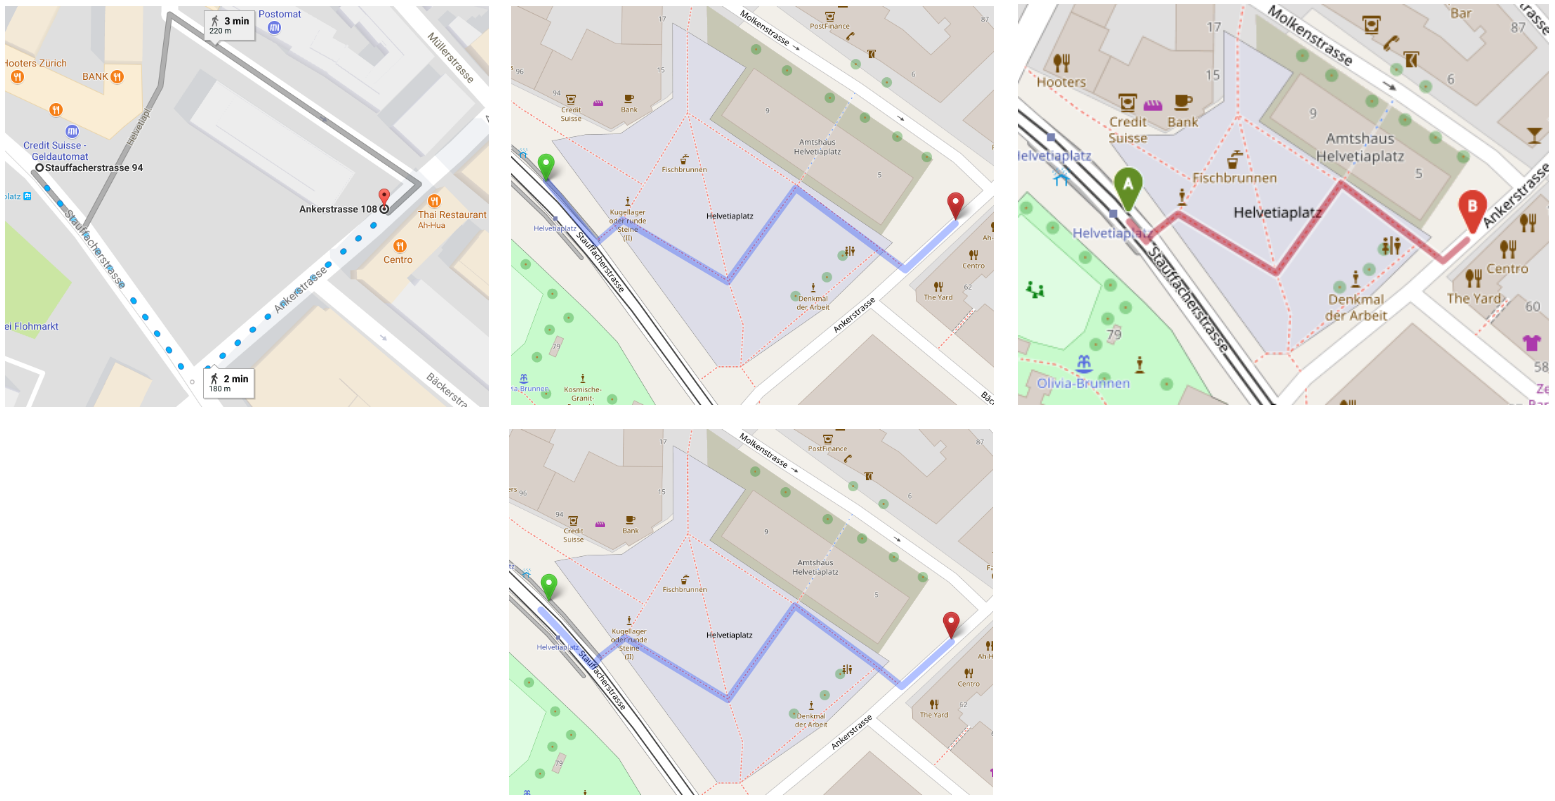
\includegraphics[width=1\linewidth]{technicalreport/img/helvetiaplatz_comparison}
\caption[Fussgänger-Routing Vergleich]{Routing-Vergleich von verschiedenen Anbietern mit Fussgänger-Profil über den Helvetiaplatz, Zürich, Schweiz; Links: Google Maps, Mitte-Oben: openstreetmap.org mit GraphHopper, Mitte-Unten: openstreetmap.org mit Mapzen, Rechts: openrouteservice.org; Screenshots aufgenommen am 13.10.2017}
\label{fig:helvetiaplatz_comparison}
\end{figure}

\begin{figure}[ht]
\centering
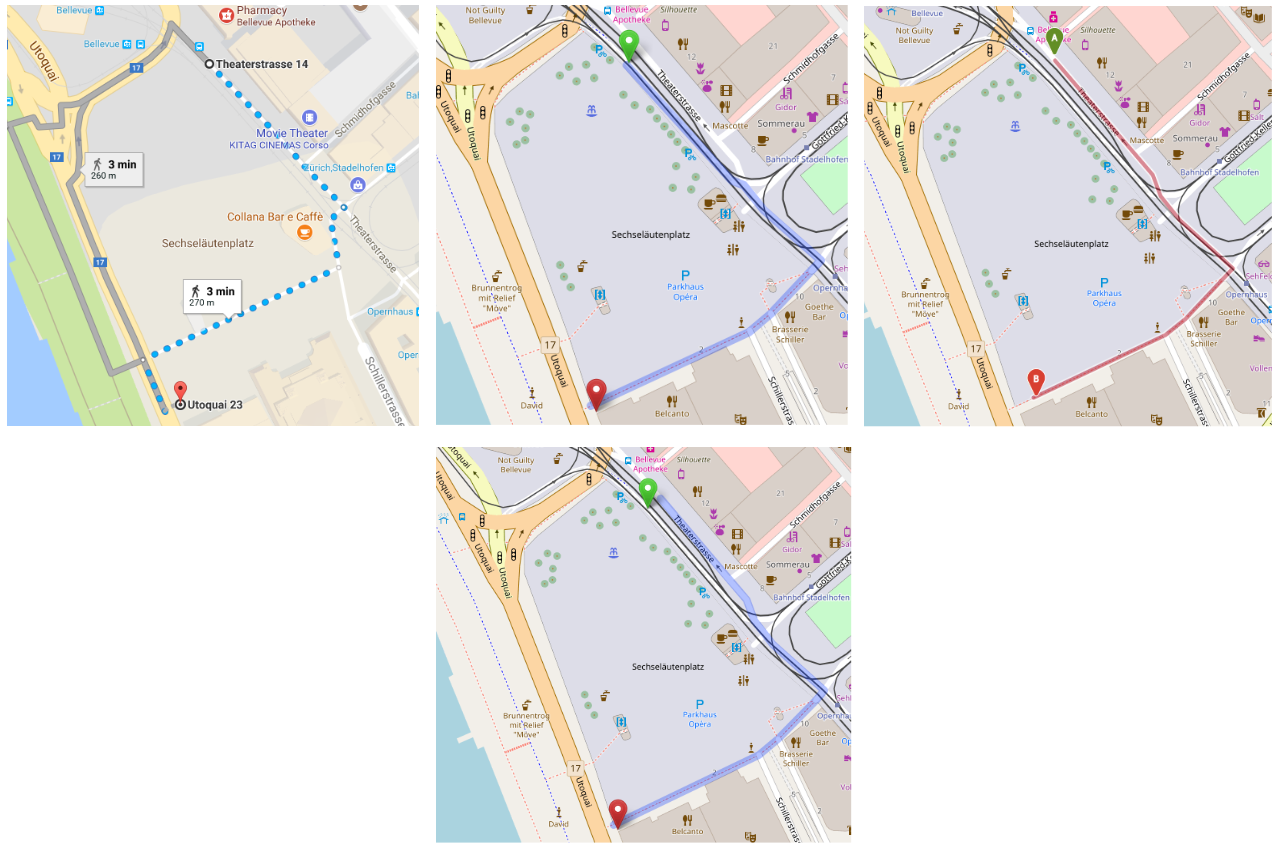
\includegraphics[width=1\linewidth]{technicalreport/img/sechselaeutenplatz_comparison}
\caption[Fussgänger-Routing Vergleich]{Routing-Vergleich von verschiedenen Anbietern mit Fussgänger-Profil über den Sechseläutenplatz, Zürich, Schweiz; Links: Google Maps, Mitte-Oben: openstreetmap.org mit GraphHopper, Mitte-Unten: openstreetmap.org mit Mapzen, Rechts: openrouteservice.org; Screenshots aufgenommen am 13.10.2017}
\label{fig:sechselaeutenplatz_comparison}
\end{figure}


Abschliessend kann man sagen, dass alle getesteten Routing-Engines mit den Fussgänger-Profilen mit Stand 13.10.2017 scheitern, wenn keine Wege über die Fläche eingezeichnet sind und so die Dauer und Streckenlänge verfälscht wird.

\subsection{Bestehende Lösungsansätze}
\label{sub:Bestehende Lösungsansätze}


\subsubsection{Routing über offene Flächen}
\label{solution:Routing über offene Flächen}

Diese Arbeit nimmt Bezug auf zwei Lösungsansätze \cite{graser_visibility_graph}, \cite{dzafic_spider_web_graph}, welche sich aus verschiedenen Motivationsgründen mit dem Problem \ref{problem:Routing über offene Flächen} befassen. Diese werden in den folgenden Unterkapitel erläutert. Mit Pseudocode wird der Ansatz verdeutlicht. Beide Varianten werden in QGIS getestet. 

Zum Schluss wird ein Variantenvergleich durchgeführt und ein Fazit gezogen. Ziel ist es, einen Flächen-Routing-Algorithmus zu finden, welche für die Vorverarbeitung der Flächen verwendet werden kann.  

\paragraph{Visibility Graph}\label{solution:Visibility Graph}~\\

Ein Ansatz zur Verhinderung von Kollisionen auf Flächen wurde in \cite{lozano-perez_visibilty_graph} als Visibility Graph beschrieben. Dabei wird in einem ersten Schritt für jeden Knotenpunkt einer Fläche eine Verbindung zu jedem anderen Knotenpunkt gezeichnet. Für unsere Zwecke werden dabei alle Knotenpunkte eines Polygons, Hindernisse,  sowie Schnittpunkte mit Strassen und Wegen (Einstiegspunkte) beachtet.
% TODO: Einheitlicher Begriff für "entry/exit points" evtl. in Begriffe definieren

In einem zweiten Schritt werden alle Verbindungen verworfen, die nicht komplett innerhalb der Fläche liegen oder mit einem Hindernis darauf kollidieren.

\begin{listing}[ht]
    \inputminted{python}{technicalreport/listing/visibility_graph_pseudocode.py}
    \caption{Konstruktion eines optimierten Visibility Graphen}
    \label{visibility_graph_pseudocode}
\end{listing}

Für die Verwendung im Routing beschreibt \cite{graser_visibility_graph} einen Ansatz, um die Kanten des Visibility Graphen zu reduzieren (siehe Listing \ref{visibility_graph_pseudocode}). Mit dem Visibility Graphen allein gäbe es mit \(n\) Knotenpunkten bis zu \(n(n-1)/2\) Kanten. Für die Reduktion wird für jeden Einstiegspunkt (wie aus Schritt 1 bekannt) jeweils der kürzeste Pfad auf dem Visibility Graphen zu allen anderen Einstiegspunkten berechnet. Alle Kanten, die nicht zu einem kürzesten Pfad gehören, werden verworfen. Abbildung  \ref{fig:visibility_graph_comparison} zeigt einen Vergleich zwischen eines Visibility Graphen vor und nach dem Reduktionsverfahren.

\begin{figure}
    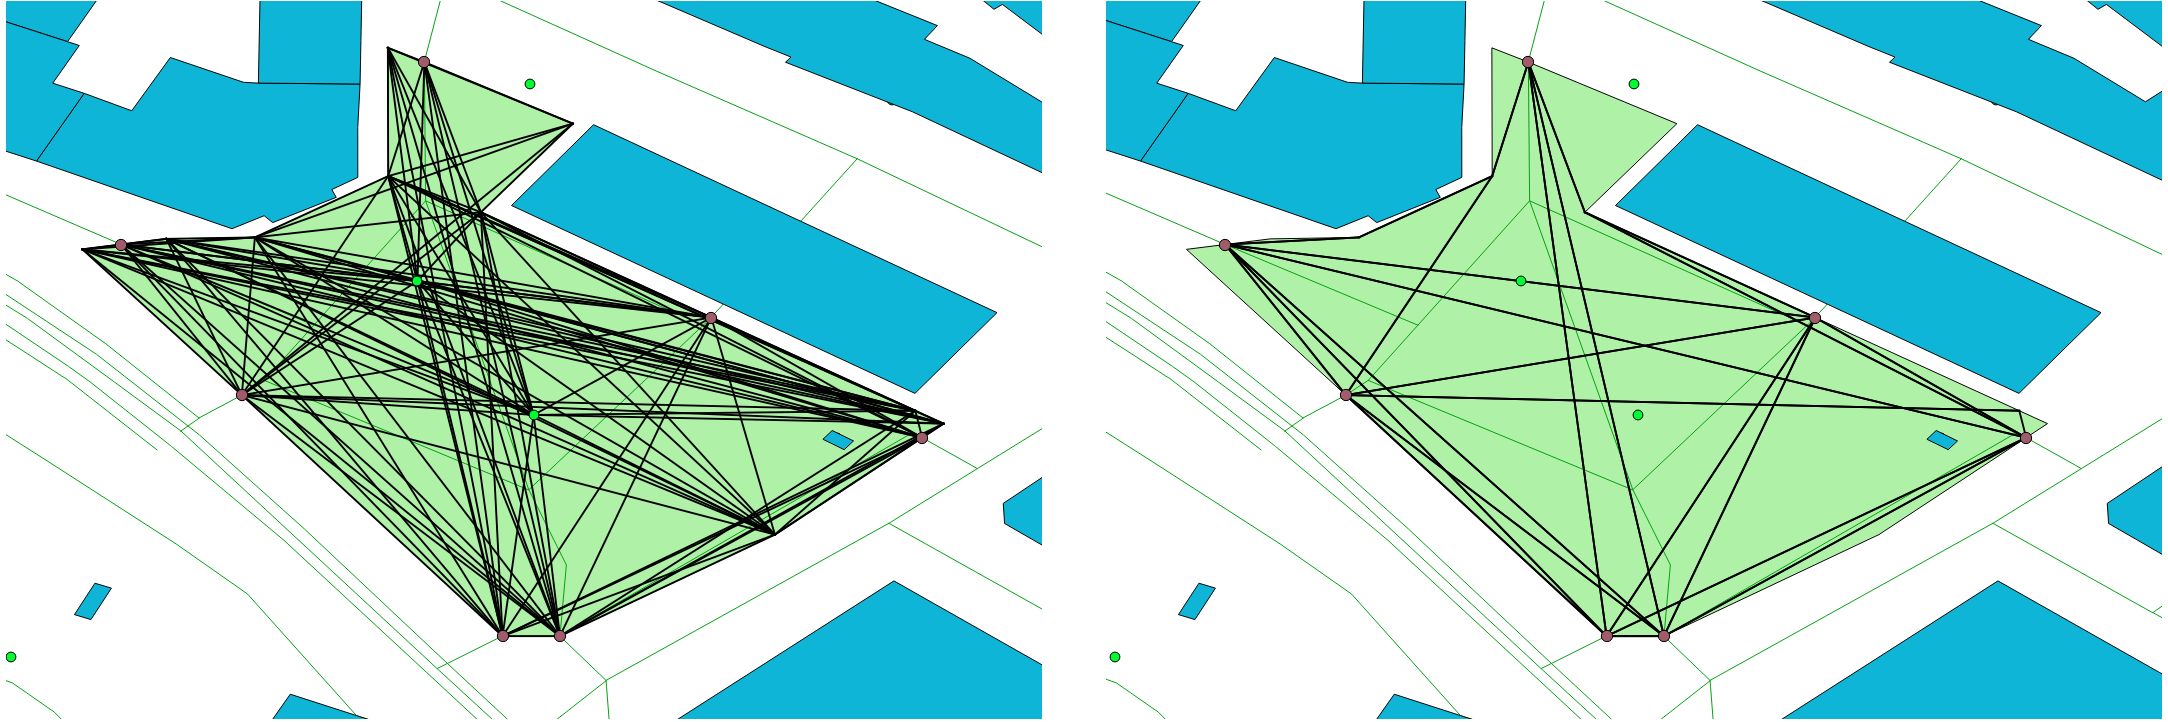
\includegraphics[width=\textwidth,keepaspectratio]{technicalreport/img/visibility_graph_comparison.png}
    \caption[Visibility Graph über Helvetiaplatz]{Visibility Graph über den Helvetiaplatz, Zürich, Schweiz; Links: Unveränderter Visibility Graph; Rechts: Reduziert auf kürzeste Pfade}
    \label{fig:visibility_graph_comparison}
\end{figure}

\paragraph{Spider-Web Graph}\label{solution:Spider-Web Graph}~\\


Die Arbeit \cite{dzafic_spider_web_graph} befasst sich mit dem Flächenrouting für Nutzern von Elektrorollstühlen, indem ein Spinnennetz (siehe Abbildung \ref{fig:spiderweb}) über das Polygon gelegt wird. Dies hat den Vorteil, dass auf dem Polygon, sprich der Fläche zusätzliche Linien und Kanten vorhanden sind, wobei statische Hindernisse berücksichtigt werden, welche für das Routing verwendet werden können. Diese Idee und das Grundprinzip wurde im folgenden übernommen.

\begin{figure}[ht]
\centering

\includegraphics[width=0.5\linewidth]{technicalreport/img/spiderweb}
\caption[Spinnennetz]{Spinnennetz}
\label{fig:spiderweb}
\end{figure}

Zur Verdeutlichung der Idee ist der Pseudocode \ref{Spiderweb Pseudocode} in zu betrachten.

\begin{listing}[ht]
    \inputminted{python}{technicalreport/listing/spiderweb_pseudocode.py}
    \caption{Spiderweb Pseudocode}
    \label{Spiderweb Pseudocode}
\end{listing}

Damit ein Spinnennetz über eine Fläche gezeichnet werden kann, muss eine Bounding-Box berechnet werden. Es handelt sich dabei um ein Rechteck, welches die ganze Fläche überdeckt. 

Vor dem Zeichnen des Spinnennetz ist es möglich, den Abstand zwischen Spalten und den Zeilen (Spacing) zu definieren. Dies hat hohe Auswirkung auf die Anzahl Zeilen und Spalten und somit auf die gezeichneten Pfade über die Fläche, da mit einem kleineren Spacing eine "Glättung" der Pfade möglich ist. Die gezeichneten Pfade widerspiegeln so eher das Verhalten eines Fussgängers. Ein Abstrich des kleiner Spacings ist sofort ersichtlich, wenn man das Spinnennetz in der Abbildung \ref{fig:spiderweb} betrachtet. Man kann annehmen, dass dieses Spinnennetz über eine Fläche von 4*4 cm mit einem Spacing von einem 1 cm gezeichnet wird. Verkleinert man nun das Spacing auf 0.5 cm, steigt die Anzahl der zu zeichnenden Linien von 72 auf 272. Halbiert man ein weiteres Mal, ist man bereits bei 1056 Linien. Damit ein Routing über das Spinnennetz und somit Abzweigungen möglich sind, kann nicht eine Line pro Zeile oder Spalte genutzt werden.

Das Zeichnen des Spinnennetzes hat eine Effizienz von \(O(NxM)\), wobei N und M die Anzahl Spalten und Zeilen sind. Die Anzahl der Zeilen und Spalten erfahren beim Halbieren des Spacings jeweils ein quadratisches Wachstum. Durch ein kleineres Spacing steigen auch die Anzahl möglicher Pfade über die Fläche an, was Auswirkung auf die Dauer der Generierung des Shortest Paths hat. 

Betrachtet man das Resultat in Abbildung \ref{fig:spiderweb_result}, sieht man in Schwarz den generierten Shortest Path über die Fläche.

\begin{figure}[th]
\centering
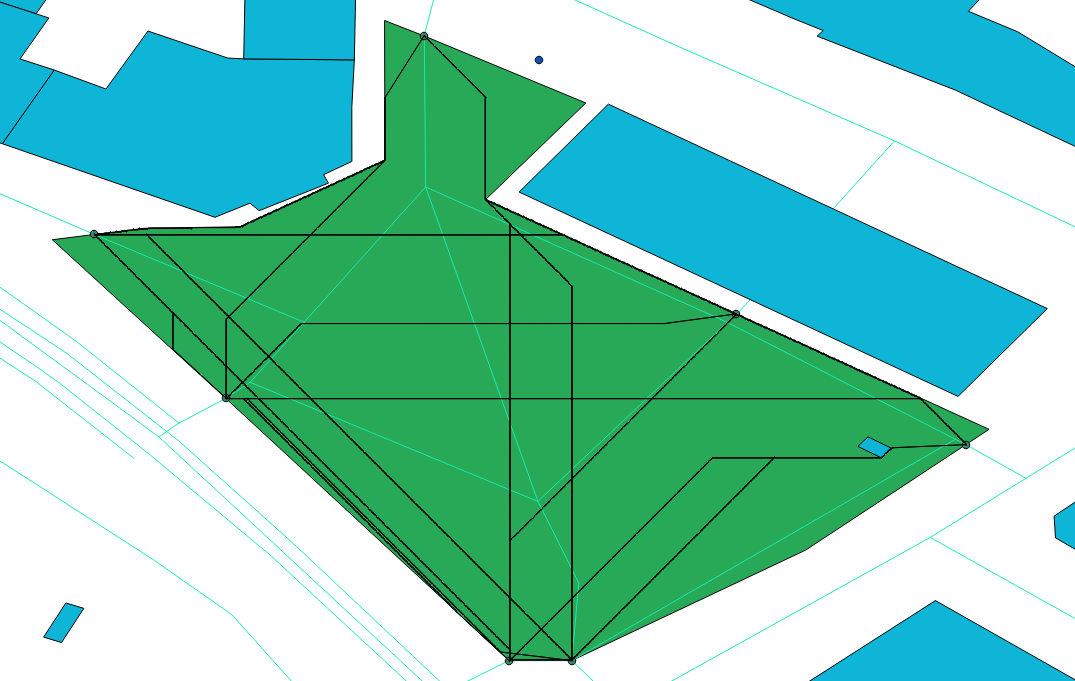
\includegraphics[width=0.7\linewidth]{technicalreport/img/spiderweb_result}
\caption[Resultat Spiderweb-Graph]{Resultat Spiderweb-Graph über Helveltiaplatz, Zürich, Schweiz}
\label{fig:spiderweb_result}
\end{figure}


Es wurde ebenfalls geprüft, ob die Rotation des Spinnennetz auf die Gegebenheit der Fläche eine Auswirkung auf die Shortest Path-Generierung hat. Bei einem Test, welcher in Abbildung \ref{fig:rotation_comparison} ersichtlich ist, wurden keine entscheidenden Vorteile gefunden, warum sich der zusätzliche Aufwand rechtfertigen würde. Das Spinnennetz wurde um 45 und um 90 Grad gedreht. Die berechneten kürzesten Pfade sind fast identisch.

\begin{figure}[th]
\centering
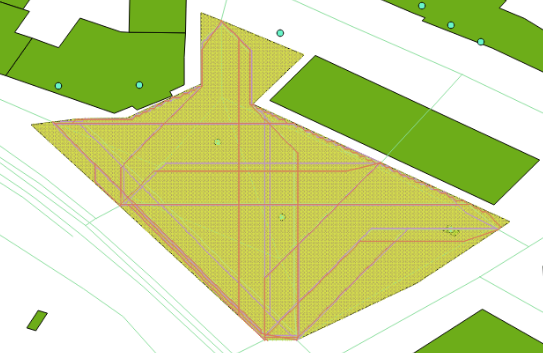
\includegraphics[width=0.7\linewidth]{technicalreport/img/rotation_comparison}
\caption[SpiderWeb-Graph Vergleich mit Rotation]{Rotation des Spiderwebs um 45 und 90 Grad im Vergleich mit keiner Rotation}
\label{fig:rotation_comparison}
\end{figure}

\paragraph{Straight Skeleton}~\\

Die Methode vom \emph{Straight Skeleton} wurde erstmals in \cite{aichholzer_skeleton} eingeführt. Dabei werden Schritt für Schritt die Kanten des Polygons zur Mitte zusammen geführt, es entstehen Verbindungen mit scharfen Ecken zu den Eckpunkten des Polygons. In Abbildung \ref{fig:skeleton_example} ist beispielhaft ein Graph aufgezeichnet.

Die Andwendung dieser Methode für Flächenrouting wurde bereits in \cite{graser_visibility_graph} diskutiert. Es stellt sich heraus, dass die \emph{Straight Skeleton} Methode keine natürlichen Routen für Fussgänger ergibt, da sie tendenziell zur Mitte der Fläche gehen und sich dabei scharfe Kurven ergeben. Aus diesen Gründen wird dieser Ansatz nicht weiter behandelt.

\begin{figure}[th]
\centering
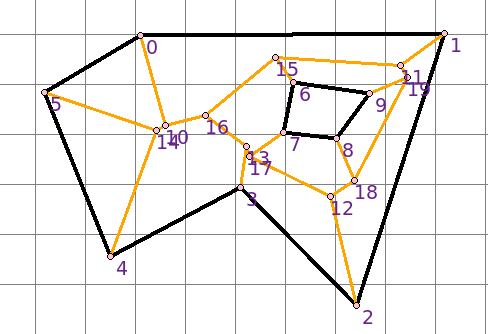
\includegraphics[width=0.7\linewidth]{technicalreport/img/skeleton_example.png}
\caption[Straight Skeleton Beispiel]{Straight Skeleton eines Multipolygons; Erstellt mit der Software pySkeleton von Ecole Centrale Paris}
\label{fig:skeleton_example}
\end{figure}

\paragraph{Einschränkungen}~\\

TODO
% TODO mögliche Einschränkungen, welche die Varianten in ihrer Anwendung betreffen

\paragraph{Vergleich}~\\

TODO
% TODO Gegenüberstellung der Varianten, welche ist in welcher Situaiton sinnvoll, wie ist der Performance-Vergleich?

\paragraph{Fazit}~\\

TODO
% TODO Welche Variante wird verwendet

\subsection{Kurzbeschreibung und Charakterisierung}
\label{sub:Kurzbeschreibung und Charakterisierung}
TODO

\subsection{Defizite}
\label{sub:Defizite}
% Hinweise auf Weiterentwicklungs-, bzw. Verbesserungspotential
TODO
% hier Probleme, welche im Visiblity Graph Paper erwähnt sind aufgreifen.
% hier Einleitung auf Optimierung der Entry Points, welche verwendet werden


\section{Bewertung}
\label{sec:Bewertung}
Im folgenden sind Komponente aufgelistet, welche im Kontext des Kapitels \ref{sec:Stand der Technik} erarbeitet wurden und einen Variantenentscheid mit sich bringen. Dazu werden messbare Kriterien definiert, gewichtet und die einzelnen Varianten daran gemessen.

Den Varianten wird eine Punktzahl auf einer linearen Skala von 1 bis 5 zugewiesen.

\subsection{Routing über offene Flächen}
\label{eval:Routing über offene Flächen}

Das Kapitel \ref{solution:Routing über offene Flächen} hat zwei Algorithmen hervorgebracht, namentlich \nameref{solution:Visibility Graph} und \nameref{solution:Spider-Web Graph}, welche im Folgenden analysiert werden.

\subsubsection{Kriterien}
\label{sub:Kriterien}

\paragraph{Verarbeitungszeit}\label{criteria:Verarbeitungszeit}~\\
Der aktuelle Import der \ac{OSM}-Daten der Schweiz ins System Tourpl \cite{hsr_tourpl}, ein Produkt des Geometa Lab der HSR \cite{geometa_lab_hsr}, dauert 2 Stunden. Diese Zeitdauer soll nicht überschritten werden. Die Verarbeitungszeit wird bewertet auf einer Skala von 1 (2 Stunden) bis 5 (0 Minuten).


\paragraph{zusätzliche Datenmenge}\label{criteria:zusätzliche Datenmenge}~\\
Die Algorithmen generieren zusätzliche Geometrien. Da die öffentlichen Plätze nur einen kleinen Teil der Kartendaten bilden, soll die zusätzliche Datenmenge keinen signifikaten Teil ausmachen. Die zusätzliche Datenmenge im Verhältnis zur originalen Datei wird bewertet auf einer Skala von 1 (1\%) bis 5 (0\%).


\paragraph{Natürlichkeit}\label{criteria:Natürlichkeit}~\\
% TODO Verweis auf Definition in Graser-Paper
Für die Natürlichkeit einer Route ist es schwer, messbare Kriterien zu definieren. Als eine natürliche Route versteht man, wenn man auf direktem Weg über den Platz geht und keine Umwege macht. Treten Hindernisse auf dem Platz auf, widerspricht es einem natürlichen Fussgänger-Verhalten, wenn man direkt aufs Hindernis zu läuft und dieses am Rande umgeht. Um trotzdem ein Fazit ziehen zu können, werden 3 Plätze (Helvetiaplatz in Zürich, Fischmarktplatz in Rapperswil-Jona und der Bahnhofplatz in Bern) untersucht. Dabei wird für beide Varianten eine interaktive Routing-Oberfläche an Probanden zu Verfügung gestellt. Die Probanden haben die Möglichkeit, selbst Routen über den Platz zu setzen. In Abbildung \ref{fig:algorithm-example-routes} sind einige Routen beispielhaft dargestellt. Danach bewerten die Probanden die vorhin definierte Natürlichkeit mit Punkten von 1 bis 5. Als massgeblicher Vergleichswert wird der Durchschnitt der Bewertungen aller Probanden genommen.

\begin{figure}[ht]
    \centering
    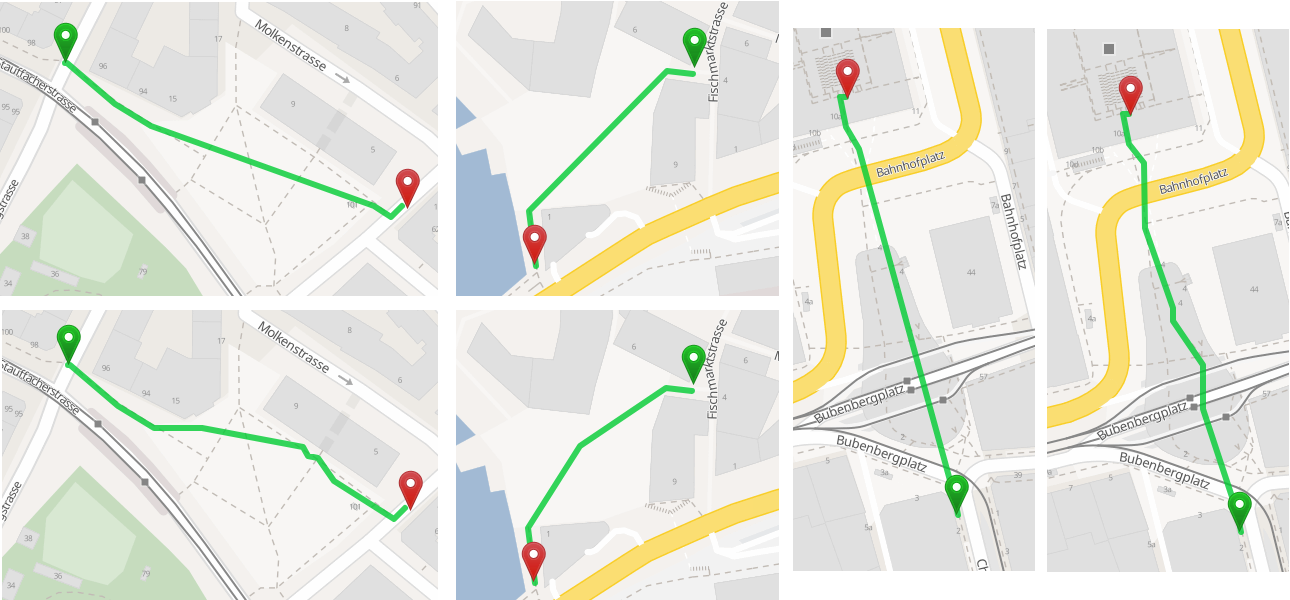
\includegraphics[width=1\linewidth]{technicalreport/img/algorithm-comparison-routes}
    \caption[Beispielhafte Routen für Natürlichkeits-Test]{Beispielhafte Routen über die drei getesteten Flächen; Jeweils oben bzw. links Visibility Graph, unten bzw. rechts Spiderweb Graph}
    \label{fig:algorithm-example-routes}
\end{figure}


\subsubsection{Resultate}
\label{sub:Resultate}

Die Vorverarbeitung wurde auf einem Rechner mit einem Intel i7 2600k Prozessor und Fedora 26 als Betriebssystem ausgeführt.

Für die Vergleichswerte der Verarbeitungszeit und der zusätzlichen Datenmenge wird die Datei \emph{switzerland-exact.osm} \cite{osm_data_switzerland}, Stand 12.11.17, verwendet. Im \ac{OSM}-Format ist die Datei 6.3 GB gross.


\begin{figure}[ht]
    \begin{tikzpicture}
        \begin{axis}[
            ybar,
            width=0.5\textwidth,
            bar width=14pt,
            ylabel={Zus. Datenmenge [MB]},
            ymin=0,
            ymax=30,
            symbolic x coords={Visibility,Spiderweb},
            xtick=data,
            enlarge x limits=0.6, % pull bars together
            nodes near coords,
            nodes near coords align={vertical},
            every node near coord/.append style={color=black}
        ] 
            \addplot[style={orange,fill=orange!30!white}]
                coordinates {(Visibility,4.1) (Spiderweb,15)};
        \end{axis}
    \end{tikzpicture}%
    ~%
    % ~ to not break the line 
    \begin{tikzpicture}
        \begin{axis}[
            ybar,
            width=0.5\textwidth,
            bar width=14pt,
            ylabel={Verarbeitungszeit [min]},
            ylabel near ticks, 
            yticklabel pos=right, % axis label on the right
            ymin=0,
            ymax=60,
            symbolic x coords={Visibility,Spiderweb},
            xtick=data,
            enlarge x limits=0.6, % pull bars together
            nodes near coords,
            nodes near coords align={vertical},
            every node near coord/.append style={color=black},
        ] 
            \addplot[style={purple,fill=purple!30!white}]
                coordinates {(Visibility,13.78) (Spiderweb,32.88)};
        \end{axis}
    \end{tikzpicture}

    \caption[Diagramm Datenmenge / Verarbeitungszeit]{Vergleich der zusätzlichen Datenmenge und der Verarbeitungszeit von Visibility Graph und Spiderweb Graph}
    \label{chart:datenmenge_laufzeit_vergleich}
\end{figure}
    

\paragraph{Verarbeitungszeit}\label{result:Verarbeitungszeit}~\\
Die Vorverarbeitung wurde mit beiden Algorithmen auf der Test-Datei ausgeführt und dabei die benötigte Zeit gemessen. Die Zeit für den ersten Schritt, das Importieren der \ac{OSM}-Daten, wird dabei abgezogen, da dies unabhängig vom jeweiligen Algorithmus ist. Die Resultate sind in Tabelle \ref{Resultat: Verarbeitungszeit} dargestellt.

\begin{table}[H]
    \centering
    \caption{Resultat: Verarbeitungszeit (ohne Initialer Import der Daten)}
    \label{Resultat: Verarbeitungszeit}
    \begin{tabular}{lll}
        & \textbf{Visiblity Graph} & \textbf{Spiderweb Graph}     \\
        Verarbeitungszeit  &        13min 47s                   & 32min 53s    \\
        %  5 - ((t / 2h)*4)
        \textbf{Bewertung 1-5} &    4.54                     &  3.90
    \end{tabular}
\end{table}


\paragraph{zusätzliche Datenmenge}\label{result:zusätzliche Datenmenge}~\\
Tabelle \ref{table: zusätzliche Datenmenge} zeigt die zusätzliche Datenmenge im \ac{OSM}-Format, die durch die Vorverarbeitung mit dem jeweiligen Algorithmus entstanden ist, verglichen mit der Dateigrösse der \ac{OSM}-Datei vor der Vorverarbeitung.

\begin{table}[H]
    \centering
    \caption{Resultat: zusätzliche Datenmenge}
    \label{table: zusätzliche Datenmenge}
    \begin{tabular}{lll}
        & \textbf{Visibility Graph} & \textbf{Spiderweb Graph} \\
        \textbf{zusätzliche Datenmenge} & 4.13 MB                    & 15.1 MB  \\  
        in Prozent der Originalgrösse   & 0.06\%                     & 0.24\%   \\
        \textbf{Bewertung 1-5}          & 4.76                       & 4.04
    \end{tabular}
\end{table}

\paragraph{Natürlichkeit}\label{result:Natürlichkeit}~\\
Für die Evaluation wurde die Bewertung der Natürlichkeit mit fünf Probanden durchgeführt. Die einzelnen Bewertungen sind in Tabelle \ref{table:Resultat Natürlichkeit} abgebildet. In Abbildung \ref{chart:natürlichkeit_vergleich} sind die durchschnittlichen Bewertungen pro Platz und Algorithmus dargestellt.

\begin{figure}[ht]
    \centering
    \begin{tikzpicture}
        \begin{axis}[
            ybar,
            width=0.8\textwidth,
            bar width=14pt,
            ylabel={Durchschnittliche Bewertung},
            ymin=1,
            ymax=5,
            symbolic x coords={Helvetiaplatz,Fischmarktplatz,Bahnhofplatz Bern},
            xtick=data,
            enlarge x limits=0.2, % pull bars together
            nodes near coords,
            nodes near coords align={vertical},
            every node near coord/.append style={color=black}
        ]            
            \addplot[style={blue, fill=blue!30!white},postaction={pattern=north east lines}] coordinates 
                {(Helvetiaplatz,3.6) (Fischmarktplatz,3.2) (Bahnhofplatz Bern,3.2)};
            \addplot [style={red, fill=red!30!white},postaction={pattern=dots}] coordinates 
                {(Helvetiaplatz,3.6) (Fischmarktplatz,3.4) (Bahnhofplatz Bern,3.2)};
            \legend{Visibility Graph,Spiderweb Graph}
        \end{axis}
    \end{tikzpicture}%

    \caption[Diagramm Natürlichkeit von Visibility / Spiderweb Graph]{Durchschnittliche Bewertungen der Natürlichkeit auf den verschiedenen Plätzen}
    \label{chart:natürlichkeit_vergleich}
\end{figure}

\begin{table}[H]
    \centering
    \caption{Resultat: Natürlichkeit}
    \label{table:Resultat Natürlichkeit}
    \begin{tabular}{lll}
        & \textbf{Visibility Graph} & \textbf{Spiderweb Graph} \\
        \textbf{Helvetiaplatz}   &                          &                          \\
        Proband 1                & 4                        & 3                        \\
        Proband 2                & 3                        & 4                        \\
        Proband 3                & 4                        & 3                        \\
        Proband 4                & 4                        & 4                        \\
        Proband 5                & 3                        & 4                        \\
        \textbf{Fischmarktplatz} &                          &                          \\
        Proband 1                & 4                        & 3                        \\
        Proband 2                & 4                        & 3                        \\
        Proband 3                & 3                        & 4                        \\
        Proband 4                & 2                        & 3                        \\
        Proband 5                & 3                        & 4                        \\
        \textbf{Bahnhofplatz Bern} &                        &                          \\
        Proband 1                & 4                        & 3                        \\
        Proband 2                & 3                        & 4                        \\
        Proband 3                & 4                        & 2                        \\
        Proband 4                & 3                        & 4                        \\
        Proband 5                & 2                        & 3                        \\
        \textbf{Resultat}        & \textbf{3.33}               & \textbf{3.4}                       
    \end{tabular}
\end{table}

\subsubsection{Auswertung und Schlussfolgerung}
\label{result:Auswertung und Schlussfolgerung}

Die einzelnen Werte sind in Tabelle \ref{table:Resultat Evaluation Flächen-Algorithmus} zusammen gefasst und gewichtet. Es zeigt sich, dass der Visibility Graph knapp besser abschneidet, der Unterschied ist allerdings sehr gering und nicht eindeutig.

Bei der Bewertung der Natürlichkeit durch Probanden ergaben sich einige Erkenntnisse. So bewerteten einige Probanden eine direkte Route mit etwas ``scharfen'' Ecken - wie sie der Visibility Graph erzeugt - natürlicher, während andere die etwas kurvigeren Routen des Spiderweb Graphs bevorzugten. Die Bewertungen der Natürlichkeit ist allerdings zu relativieren, da fünf Probanden in diesem Kontext nicht ausreichen, um eine abschliessende Erkenntnis zu gewinnen. Für einen ersten Eindruck genügt dies aber.

Abschliessend kann man sagen, dass beide Algorithmen gute Resultate bringen. Wenn die Verarbeitungszeit wichtig ist, bringt der Visibility Graph Vorteile, der Spiderweb Graph erzeugt dafür tendenziell die etwas natürlicheren Routen.

\begin{table}[ht]
    \centering
    \caption{Resultat der Evaluation Flächen-Algorithmus}
    \label{table:Resultat Evaluation Flächen-Algorithmus}
    \begin{tabular}{lllll}
            \hline
            \textbf{ID} & \textbf{Titel}         & \textbf{\begin{tabular}[c]{@{}l@{}}Relatives Gewicht \\ (0-1)\end{tabular}} & \textbf{Visibility Graph} & \textbf{Spiderweb Graph} \\ \hline
            1           & \nameref{criteria:Verarbeitungszeit}      & 0.3       & 4.54 / 1.36                   & 3.9 / 1.17                   \\
            2           & \nameref{criteria:zusätzliche Datenmenge} & 0.2       & 4.76 / 0.95                   & 4.04 / 0.81                  \\
            3           & \nameref{criteria:Natürlichkeit}          & 0.5       & 3.33 / 1.67                   & 3.4 / 1.7                    \\ \hline
            \multicolumn{3}{l}{\textbf{Total}}                                  & \textbf{12.6 / 3.98}         & \textbf{11.36 / 3.68}
     \end{tabular}               
\end{table}



\section{Umsetzungskonzept}
\label{sec:Umsetzungskonzept}
TODO

\subsection{Beschreibung des eigenen Lösungskonzepts}
\label{sub:Beschreibung des eigenen Lösungskonzepts}
% z.T. Wiederholung im Groben, z.T. Verweise auf Teil II-Kapitel
TODO


\section{Resultate}
\label{sec:Resultate}

In diesem Kapitel werden die Resultate der Arbeit präsentiert. Die technische Beschreibung zur Implementation befindet sich in Teil \ref{chap:SW-Projektdokumentation} Kapitel \ref{sec:Implementation}.

\subsection{Zielerreichung}
\label{sub:Zielerreichung}

In der Evaluations-Phase wurde der Stand der Technik analysiert (Kap. \ref{sec:Stand der Technik}). Mit ersten Tests und Proof-of-Concept Implementationen in QGIS konnten dabei die Stärken und Schwächen der jeweiligen Algorithmen heraus gearbeitet werden. Es stellte sich schnell heraus, dass die beiden Ansätze \nameref{solution:Visibility-Graph} und \nameref{solution:SpiderWeb-Graph} sich am besten für unser Problem eignen. Parallel dazu wurden die Umsysteme analysiert, die für unsere Problemstellung eines multimodalen Routings benötigt werden (siehe Teil \ref{chap:SW-Projektdokumentation} Kap. \ref{sec:Analyse}). Dazu gehörte eine Analyse bestehender Routing-Engines und das Finden der ÖV-Haltestellen im näheren Umkreis.

Im nächsten Schritt wurden die Vorverarbeitung von \ac{OSM}-Daten mit der Flächenoptimierung implementiert. Die beiden Algorithmen --- \nameref{solution:Visibility-Graph} und \nameref{solution:SpiderWeb-Graph} --- wurden dabei parallel implementiert. Dies ermöglichte es uns, beide Ansätze optimal miteinander zu vergleichen (siehe Kapitel \ref{sec:Bewertung Routing über offene Flächen}).

Zusammen mit der Vorverarbeitung haben wir einen Service \cite{github:PlazaRoute} implementiert, der mit Hilfe der Routing-API von search.ch \cite{search_ch_route_api} ein Routing mit öffentlichen Verkehrsmitteln ermöglicht, wobei für das Fussgänger-Routing unsere optimierten Daten der Vorverarbeitung verwendet werden, um ein natürliches Fussgänger-Routing über offene Flächen zu erreichen. Dabei werden von einem beliebigen Startpunkt aus mehrere Haltestellen in der Umgebung gesucht und mit der Kombination von Fussgänger- und ÖV-Routing die optimale Route ermittelt.

Die Koordinaten der \glspl{Kante} werden dabei so optimiert, dass die Kante in die richtige Fahrtrichtung angesteuert werden kann.

Damit unser Service getestet und visualisiert werden kann, wurde ein Plugin für QGIS entwickelt \cite{github:PlazaRoute-qgis-plugin}. Dieses ermöglicht es, mit unserem Service Routen für den öffentlichen Verkehr interaktiv zu berechnen und visualisieren.

\subsection{Ausblick: Weiterentwicklung}
\label{sub:Ausblick: Weiterentwicklung}

Die von uns implementierte Vorverarbeitung für \ac{OSM}-Daten kann als Referenz dienen, um in Zukunft die Optimierung für Fussgänger-Flächen in bestehende Routing-Engines einzubauen. Es wäre sinnvoll, die Algorithmen direkt in Routing-Engines zu integrieren, statt in einem sepparaten Schritt zuerst \ac{OSM}-Daten aufbereiten zu müssen.

Die jetzige Lösung bietet noch weiteren Raum für Optimierung. So können im Moment einige Plätze nicht verarbeitet werden, weil zu wenig \glspl{Einstiegspunkt} existieren, obwohl in der Realität der Platz problemlos begehbar wäre. Ein ähnliches Problem besteht auch, wenn mehrere Fussgänger-Flächen direkt aneinander liegen. Ansätze für Lösungen dazu werden in den Kapiteln \ref{subsub:Verbesserung_Einstiegspunkte} respektive \ref{subsub:Routing bei zwei benachbarten Flächen} diskutiert.

Die jetzige Lösung mit Python stösst mit der Performanz an ihre Grenzen. Es ist denkbar, eine Lösung mit PostGIS oder C++ zu realisieren.

\subsection{Persönliche Berichte}
\label{sub:Persönliche Berichte}

\subsubsection{Robin Suter}
\label{Persönliche Berichte:Robin Suter}
Schon seit geraumer Zeit interessiere ich mich für Algorithmen für die Analyse von Graphen. Diese Arbeit bot mir eine gute Möglichkeit, dies auf ein praktisches Problem anwenden zu können. Die Struktur mit dem grossen theoretischen Teil gefiel mir gut, da es mir neben dem Software-Engineering auch eine Möglichkeit gab, mich wissenschaftlich mit einem Thema zu befassen.

Es war sehr motivierend, mit den \ac{OSM}-Daten zu arbeiten und damit die Vorverarbeitung zu implementieren. Dabei konnte ich auch schön beobachten, wie eine kleine Optimierung in der Komplexität einen sehr grossen Unterschied in der Laufzeit ausmachen kann.

Die Datenqualität der Kartendaten war eine Herausforderung, wir entdeckten immer wieder neue Grenzfälle, die in die Verarbeitung einbezogen werden mussten. Dies motivierte aber auch immer, unseren Code zu optimieren.

Die Zusammenarbeit im Team funktionierte stets sehr gut. Der gegenseitige Austausch war sehr hilfreich, um gemeinsam Problemlösungen zu finden und Ideen auszutauschen.

Insgesamt bin ich sehr zufrieden mit dieser Arbeit. Ich hoffe, dass unsere Software in Zukunft von der Open-Source-Community weiter verwendet werden kann, um das Routing zu verbessern.


\subsubsection{Jonas Matter}
\label{Persönliche Berichte:Jonas Matter}
Die Themengebiete Pfadoptimierung und \ac{GIS} begeistern mich seit einiger Zeit. Eine Arbeit in diesem Bereich schreiben zu dürfen, kam somit gelegen. PlazaRoute unterscheidet sich im Aufbau von meinen bisher durchgeführten Software-Projekten. Die Arbeit hat einen grossen theoretischen Fokus und war unter anderem geprägt von viel Wissensaufbau im Bereich der Flächenverarbeitungsalgorithmen und des Routings. 

Der Umgang mit grossen Datenmengen war eine Herausforderung, die spannend zu lösen war. Es war interessant zu sehen, was kleine Anpassungen für grosse Performanzgewinne mit sich bringen können.

Die Zusammenarbeit mit Robin Suter war wie auch in vorherigen Projekten eine Bereicherung. Die gegenseitigen Reviews und das Hinterfragen der Lösungen regten zum Reflektieren an und haben zu einer hohen Qualität beigetragen, sei dies auf Seiten der Architektur, des Codes oder der Dokumentation.

Abschliessend kann ich sagen, dass ich mit dem Verlauf und dem Resultat der Arbeit sehr zufrieden bin und hoffe, dass PlazaRoute in der einen oder anderen Art dem Fussgänger zu gute kommen wird.


\subsection{Dank}
\label{sub:Dank}

Wir möchten folgenden Personen für ihre Unterstützung und Mitwirkung bei dieser Arbeit danken:

\textbf{Prof. Stefan Keller, IFS Institut für Software,} für die Zeit, Ressourcen, Kontakte, Know-How und Unterstützung, von welcher wir jederzeit profitieren konnten.

\textbf{Christian Helbling, localsearch,} für den Erfahrungsaustausch im Bereich der Fahrplandaten und search.ch.

\textbf{Prof. Dr. Olaf Zimmermann, IFS Institut für Software,} für die wertvolle Expertise in Sachen Software-Architektur.

\textbf{Mitarbeiter, IFS Institut für Software,} für den regen Know-How-Austausch und die Unterstützung bei der Produktivsetzung.


% Summary index document for ...

\chapter{SW-Projektdokumentation }
\label{chap:SW-Projektdokumentation}

\section{Überblick}
\label{sec:Überblick}
Das Kapitel \nameref{chap:Technischer Bericht} verfolgt das Ziel, dem Leser eine Überblick über die Problemstellung zu geben und was Inhalt der Arbeit ist. Dabei wurde dem \nameref{sec:Stand der Technik} besondere Beachtung geschenkt. Das Kapitel \nameref{chap:SW-Projektdokumentation} legt den Fokus auf die konkrete Umsetzung von PlazaRoute.

\section{Vision}
\label{sec:Vision}
% Evtl. direkt auf Kapitel 1.1.1 verweisen

TODO
\section{Anforderungsspezifikation}
\label{sec:Anforderungsspezifikation}

\subsection{Use Cases}
\label{sub:Use Cases}
Im folgenden sind die funktionalen Anforderungen an PlazaRoute mit all seinen Komponenten, welche im Kapitel \ref{sec:Architektur} aufgeführt sind, als Use Cases im Brief-Format beschrieben. Zur Übersicht ist das Use Case Diagramm in Abbildung \ref{fig:usecase_diagram} zu betrachten.

\begin{figure}[ht]
\centering
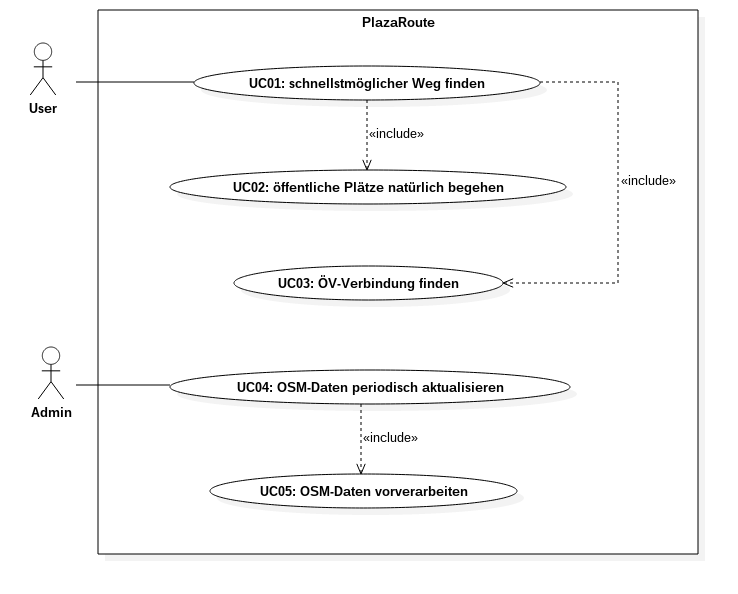
\includegraphics[width=1\linewidth]{projectdoc/img/usecase_diagram}
\caption[Use Case Diagramm]{Use Case Diagramm}
\label{fig:usecase_diagram}
\end{figure}

\subsubsection{Aktoren}
\label{useccase:Aktoren}

\begin{table}[h]
    \centering
    \caption{Aktoren}
    \label{aktoren}
    \begin{tabular}{ll}
        \textbf{Aktor} & \textbf{Beschreibung und Interessen}                                                                                                                                                                                     \\
        \textbf{User}  & \begin{tabular}[c]{@{}l@{}}Ein User ist ein Fussgänger, welcher schnellstmöglich von Punkt A zu Punkt B kommen möchte. \\ Er fungiert in der Komponente QGIS-Plugin.\end{tabular}                                          \\
        \textbf{Admin} & \begin{tabular}[c]{@{}l@{}}Ein Admin ist daran interessiert, dass aktuelle Daten dem Aktor User zur Verfügung stehen. \\ So möchte er Daten vorverarbeiten und dem Aktor User diese zur Verfügung stellen können.\end{tabular}
    \end{tabular}
\end{table}

\subsubsection{UC01: schnellstmöglicher Weg finden}
\label{usecase:UC01}
Aktoren: \emph{User}

Include: \nameref{usecase:UC02}, \nameref{usecase:UC03}

Nachdem der User einen Start- und Endpunkt (geografische Standorte) angegeben hat, erhält er den schnellstmöglichen Weg, welcher mit öffentlichen Verkehrsmitteln und zu Fuss machbar ist.

\subsubsection{UC02: Flächen im urbanen Raum natürlich begehen}
\label{usecase:UC02}
Aktoren: \emph{User}

Der User wird beim Fussgänger-Routing über Flächen im urbanen Raum auf direktem Weg natürlich (Definition im Kapitel \ref{criteria:Natürlichkeit} im Teil \ref{chap:Technischer Bericht}) geroutet. Dies betrifft insbesondere das Umgehen von Hindernissen.

\subsubsection{UC03: ÖV-Verbindung finden}
\label{usecase:UC03}
Aktoren: \emph{User}

Der User wird zu Fuss zu einer ÖV-Haltestelle geroutet, welche sich in einem Umkreis von 1 km befindet. Falls mehrere ÖV-Haltestellen verfügbar sind, wird die ÖV-Haltestelle gewählt, welche die kürzeste Reisezeit (Fussweg + ÖV-Weg) hat.

\subsubsection{UC04: OSM-Daten periodisch aktualisieren}
\label{usecase:UC04}
Aktoren: \emph{Admin}

Include: \nameref{usecase:UC05}

Der Admin aktualisiert die \ac{OSM}-Daten, auf welche in \nameref{usecase:UC01} geroutet wird, periodisch und integriert sie in die \gls{Routing-Engine}.

\subsubsection{UC05: OSM-Daten vorverarbeiten}
\label{usecase:UC05}
Aktoren: \emph{Admin}

Der Admin führt die Vorverarbeitung der \ac{OSM}-Daten durch. Unter Vorverarbeitung versteht man das Einzeichnen von Fusswegen auf Flächen im urbanen Raum. Diese Daten werden der \gls{Routing-Engine} übergeben und ermöglicht, dass die Routing-Engine den schnellstmöglichen Weg über Flächen im urbanen Raum finden kann.

\subsection{Nicht-funktionale Anforderungen}
\label{sub:Nicht-funktionale Anforderungen}

\subsubsection{NFA01: Docker-Images}
\label{NFA:NFA01}

PlazaRoute wird in Docker-Images ausgeliefert, um eine Verfügbarkeit auf unterschiedlichen Systemen sicherstellen und um das Deployment vereinfachen zu können.

\subsubsection{NFA02: austauschbare \gls{Routing-Engine}}
\label{NFA:NFA02}

Die \gls{Routing-Engine}, welche von PlazaRoute verwendet wird, soll austauschbar sein. Dabei soll nur die konkrete Implementation des Services, welche fürs Routing genutzt wird, angepasst werden müssen.

\subsubsection{NFA03: periodische Aktualisierung der OSM-Daten}
\label{NFA:NFA03}

Die \ac{OSM}-Daten werden wöchentlich für ein optimiertes Fussgänger-Routing über Flächen im urbanen Raum vorverarbeitet und der Routing-Engine übergeben.


\subsubsection{NFA04: Dauer der Vorverarbeitung}
\label{NFA:NFA04}

Die Vorverarbeitung der \ac{OSM}-Daten (Optimierung auf Flächen im urbanen Raum) darf maximal 2 Stunden dauern.

\subsubsection{NFA05: zusätzliche Datenmenge}
\label{NFA:NFA05}

Die zusätzlichen Daten für die Optimierung (zusätzlich eingezeichnete Wege über Flächen im urbanen Raum) dürfen nicht mehr als 1\% des Kartenmaterials betragen.

\subsubsection{NFA06: Dauer des Unterbruchs bei OSM-Daten-Integration}
\label{NFA:NFA06}

PlazaRoute ist während dem Integrieren der neuesten \ac{OSM}-Daten in die \gls{Routing-Engine} maximal 2 Stunden nicht verfügbar. Der User wird nicht über den Unterbruch informiert.

\section{Analyse}
\label{sec:Analyse}

In diesem Kapitel werden Abhängigkeiten und Umsysteme analysiert, die potentiell benötigt werden. Neben der Evaluation der Routing-Engine (\ref{analyse:Evaluation Routing-Engine}) gehören Overpass (\ref{analyse:nächste ÖV-Haltestellen finden}) und search.ch (\ref{analyse:Search.ch Anbindung}) zu den wichtigsten Systemen in unserer Applikation.

\subsection{Evaluation Routing-Engine}
\label{analyse:Evaluation Routing-Engine}
Eine Evaluation der gängigen \ac{OSM}-Routing-Engines wurde in \cite{eval_routing_engine} ausgiebig durchgeführt. Bei unserer Evaluation beschränken wir uns auf die drei "grössten" Routing-Engines \emph{OSRM}\cite{osrm}, \emph{Valhalla}\cite{valhalla} und \emph{Graphhopper}\cite{graphhopper}. Die Auswahl fiel auf diese drei, weil sie von den in \cite{eval_routing_engine} evaluierten Routing-Engines anhand der Github-Metriken mit Abstand die grösste Verbreitung haben.

Bei einem Test mit einer von uns vorverarbeiteten \ac{OSM}-Datei gab es bei \emph{Valhalla} sofort Probleme, weil wir negative \ac{OSM}-IDs verwenden, um Konflikte mit bestehenden Daten zu vermeiden. Für die weitere Evaluation beschränken wir uns daher auf die beiden Routing-Engines \emph{Graphhopper} und \emph{OSRM}.

Die Engines werden an folgenden Kriterien gemessen:

\subsubsection{Infrastruktur-Integration}
\label{analyse:Infrastruktur-Integration}
Es wird analysiert, wie einfach die Routing-Engine aufgesetzt werden kann. Ziel ist es, dass die Routing-Engine in einem eigenen Docker-Image (siehe \nameref{NFA:NFA01}) auf dem Server läuft.

\emph{Graphhopper} und \emph{OSRM} sind bereits als Docker-Image verfügbar und können somit einfach auf einem beliebigen Server gestartet und verwendet werden.


\subsubsection{Applikation-Anbindung}
\label{analyse:Applikation-Anbindung}
Da mit der Routing-Engine kommuniziert werden muss, wird geprüft, wie einfach die Routing-Engines an eine Applikation angebunden werden können.

Beide Routing-Engines bieten zusätzlich ein fertiges HTTP-Backend an, welches für das Routing genutzt werden kann. Somit können beide Routing-Engines auf die gleiche Art und Weise eingebunden werden.

\subsubsection{OSM-Daten-Integration}
\label{analyse:OSM-Daten-Integration}
Für die Flächentraversierung müssen eigene \ac{OSM}-Daten generiert werden. Diese vorverarbeiteten \ac{OSM}-Daten müssen für das Fussgänger-Routing der Routing-Engine übergeben werden.

Sowohl \emph{OSRM} als auch \emph{Graphhopper} können beim Starten der Graphen-Aufbereitung eine \ac{OSM}-Datei übergeben werden.

\subsubsection{Geschwindigkeit der Vorverarbeitung}
\label{analyse:Geschwindigkeit der Vorverarbeitung}
Die von uns erzeugte \ac{OSM}-Datei wird der Routing-Engine zur Verarbeitung übergeben, um daraus einen Routing-Graphen zu generieren. Da dieser Prozess für jeden Durchlauf unserer Plaza-Vorverarbeitung aufs Neue geschehen muss, soll dies möglichst schnell sein.

Bei einem Test mit einer von uns vorverarbeiteten OSM-Datei brauchte \emph{Graphhopper} nur wenige Minuten, während \emph{OSRM} über 30 Minuten für die Verarbeitung beanspruchte.

\subsubsection{Konfigurationsmöglichkeiten}
\label{analyse:Konfigurationsmöglichkeiten}
Für unsere Zwecke ist es sinnvoll, wenn wir die Routing-Engines auf das Fussgänger-Routing konfigurieren können. So sind z.B. Contraction Hierarchies nicht notwendig, da wir keine grossen Routen berechnen.

\emph{Graphhopper} bietet die meisten Konfigurationsmöglichkeiten. Contraction Hierarchies können deaktiviert werden und für die Shortest-Path-Berechnung werden die A*- und Dijkstra-Algorithmen \cite{astar} \cite{dijkstra_algorithm} unterstützt. \emph{OSRM} bietet ebenfalls einen Modus ohne Contraction Hierarchies, allerdings nur mit dem Dijkstra-Algorithmus.

\subsubsection{Fussgänger-Profil}
\label{analyse:Fussgänger-Profil}
Für das Routing werden bestimmte Profile verwendet, um das Routing auf verschiedene Transportarten wie Auto oder Fussgänger zu optimieren. Für uns ist es von Vorteil, wenn eine Routing-Engine bereits ein vorkonfiguriertes Profil für Fussgänger mitbringt.

\emph{Graphhopper} und \emph{OSRM} bringen beide bereits ein vorkonfiguriertes Fussgänger-Profil mit.

\subsubsection{Resultat}
\label{analyse:Resulat}
Bezüglich der Integration unterscheiden sich \emph{Graphhopper} und \emph{OSRM} kaum. Der Entscheid fiel auf \emph{Graphhopper}, da die Vorverarbeitung deutlich schneller ist und die Konfigurationsmöglichkeiten uns mehr Freiheiten bieten. Mit der Auswahl zwischen Dijkstra \cite{dijkstra_algorithm} und A* \cite{astar} können wir auch vergleichen, welcher Algorithmus besser für Flächen-Traversierungen geeignet ist.


\subsection{nächste ÖV-Haltestellen finden}
\label{analyse:nächste ÖV-Haltestellen finden}

Das grundlegende Ziel ist es, von einem Startpunkt aus eine Destination zu Fuss und mit dem öffentlichen Verkehr zu erreichen. Dabei sollen die ÖV-Haltestellen in einem zu Fuss machbaren Umkreis berücksichtigt werden. Von diesen ÖV-Haltestellen ausgehend wird das ÖV-Routing an die Zieldestination durchgeführt.

Für die Anforderung \ref{target:nächste ÖV-Haltestellen finden} bietet sich Overpass an. Overpass ermöglicht es, über eine umfassende \ac{API} selektiv Daten von \ac{OSM} zu beziehen. Dabei besteht die Option, die Overpass \ac{QL} oder XML-Abfragen zu verwenden. Die Suche lässt sich nach allem einschränken, was der Mapper in den \ac{OSM}-Daten spezifizieren kann. So ist das Filtern nach Objekttyp, Keys, Tags, etc. unbeschränkt möglich und bietet so eine hohe Flexibilität. Overpass liefert die Resultate als JSON-Objekt oder XML. 

Für eine einfache Intergration in Python gibt es Overpass Wrapper. Dabei wurden zwei Libraries berücksichtigt, namentlich \emph{overpass-api-python-wrapper} und \emph{OverPy}. Die Libraries haben einen ähnlich häufigen Updatezyklus. Für beide wurde ein Proof of Concept implementiert, welcher die ÖV-Haltestellen im einem kleinen Umkreis vom Stadelhofen, Zürich, Schweiz abfragt.

Die Entscheidung fiel dabei auf OverPy. Ausschlaggebend war die ausführlichere Dokumentation und dass OverPy Klassen für Nodes, Relations, Way, Area, etc. und Hilfsfunktionen, welche das Ganze übersichtlich halten, anbietet. Bei \emph{overpass-api-python-wrapper} besteht der Nachteil, dass das JSON-Resultat der Abfrage selber geparsed und verarbeitet werden muss.

\begin{listing}[ht]
    \inputminted{python}{projectdoc/listing/get_public_transport_stops_overpass.py}
    \caption{ÖV-Haltestellen von \acs{OSM} mit Overpass beziehen}
    \label{get_public_transport_stops_overpass}
\end{listing}

In Listing \ref{get_public_transport_stops_overpass} ist zu sehen, wie für eine Bounding Box, welche im Süden durch den minimalen Breitengrad, im Westen durch den minimalen Längengrad, im Norden durch den maximalen Breitengrad und im Osten durch den maximalen Längengrad begrenzt ist, die ÖV-Haltestellen abgefragt werden. Dabei wird die JSON-Response in Node-Objekte geparsed, welche weiterverwendet werden können. In diesem Beispiel wird für die Abfrage die erwähnte Overpass QL verwendet.

Es ist ebenfalls möglich, eine Umkreissuche mit \code{around} durchzuführen. Dies hat Performance-Nachteile und es gibt keine entscheidenden Gründe, warum es vorteilhafter sein sollte, wenn man einen Kreis statt ein Rechteck um einen Ausgangspunkt zieht.

\subsection{Search.ch Anbindung}
\label{analyse:Search.ch Anbindung}
Search.ch bietet für Fahrplan-Abfragen eine API \cite{search_ch_route_api} an. So ist  auch eine ÖV-Routensuche möglich. Diese ist zum aktuellen Zeitpunkt unter \cite{search_ch_route_api} verfügbar und nimmt die in Tabelle \ref{search_ch_route_api_specification} spezifizierten und für uns relevanten Parameter entgegen. In einer ersten Version wird nur \code{from} und \code{to} verwendet.

\begin{table}[ht]
    \centering
    \caption{Search.ch Route API Spezifikation; Teilauszug von \cite{search_ch_route_api}}
    \label{search_ch_route_api_specification}
    \begin{tabular}{lllll}
        \textbf{Parameter}   & \textbf{Zwingend} & \textbf{Beschreibung}                                                                & \textbf{Beispiel}          & \textbf{Default} \\
        \code{from}       & \code{true}              & Abfahrtsstation                                                                      & Zürich, Sternen Oerlikon   &                  \\
        \code{to}         & \code{true}              & Abfahrtsstation                                                                      & Zürich, Hallenbad Oerlikon &                  \\
        \code{date}       & \code{false}             & Datum                                                                                & 29.10.2017                 & today            \\
        \code{time}       & \code{false}             & Zeit                                                                                 & 15:00                      & now            \\
        \code{time\_type} & \code{false}             & \begin{tabular}[c]{@{}l@{}}date/time als Abfahrts-  \\ oder Ankunftszeit\end{tabular} & arrival                    & depart
    \end{tabular}
\end{table}

Also Antwort erhält man ein JSON-Objekt, welches eine Liste an möglichen Verbindungen beinhaltet. In einer zurückgelieferten Verbindung sind alle Teilstrecken definiert. Die erste Teilstrecke bestimmt den Ausgangspunkt der ÖV-Verbindung. Diese ist von besonderer Relevanz. In \ref{problem:mehrere Kanten mit dem gleichen Namen} wurde aufgezeigt, dass es normalerweise mehrere \glspl{Kante} mit dem gleichen Namen geben kann und nun zur richtigen geroutet werden muss. So kann mithilfe von der \code{stopid}, welche dem \acs{OSM}-Tag \code{uic\_ref} entspricht, und \code{terminal} die richtige Kante ermittelt werden. Man kann mithilfe von Overpass die ÖV-Linien der Teilstrecke laden. Die letzte ÖV-Haltestelle der Linie muss nun dem Wert in \code{terminal} entsprechen. Dadurch hat man die ÖV-Linie in die richtige Fahrtrichtung ermittelt und kann so die Ausgangskante auf dieser Linie extrahieren. Das Gleiche trifft natürlich auf die Endkante der Verbindung zu.

\subsubsection{Einschränkungen}
\label{analyse:search.ch Einschränkungen}
Die Anzahl täglicher Anfragen ist für den freien Gebrauch auf 1000 beschränkt.


\section{Architektur}
\label{sec:Architektur}

In diesem Kapitel wird die Architektur unserer Applikation und die Schnittstellen zu den Umsystemen besprochen. Als Anhaltspunkt wird das C4 Modell \cite{c4model} von Simon Brown verwendet. In einem ersten Schritt wird unsere Applikation in den Kontext des grösseren Systems gesetzt. Anschliessend teilen wir das System \emph{PlazaRoute} in einzelne Container und den zentralen Container \emph{Plaza Routing} in einzelne Komponenten auf.

\subsection{Systemkontext}
\label{architektur:Systemkontext}

\begin{figure}[ht]
\centering
% TODO: Grafik zuschneiden
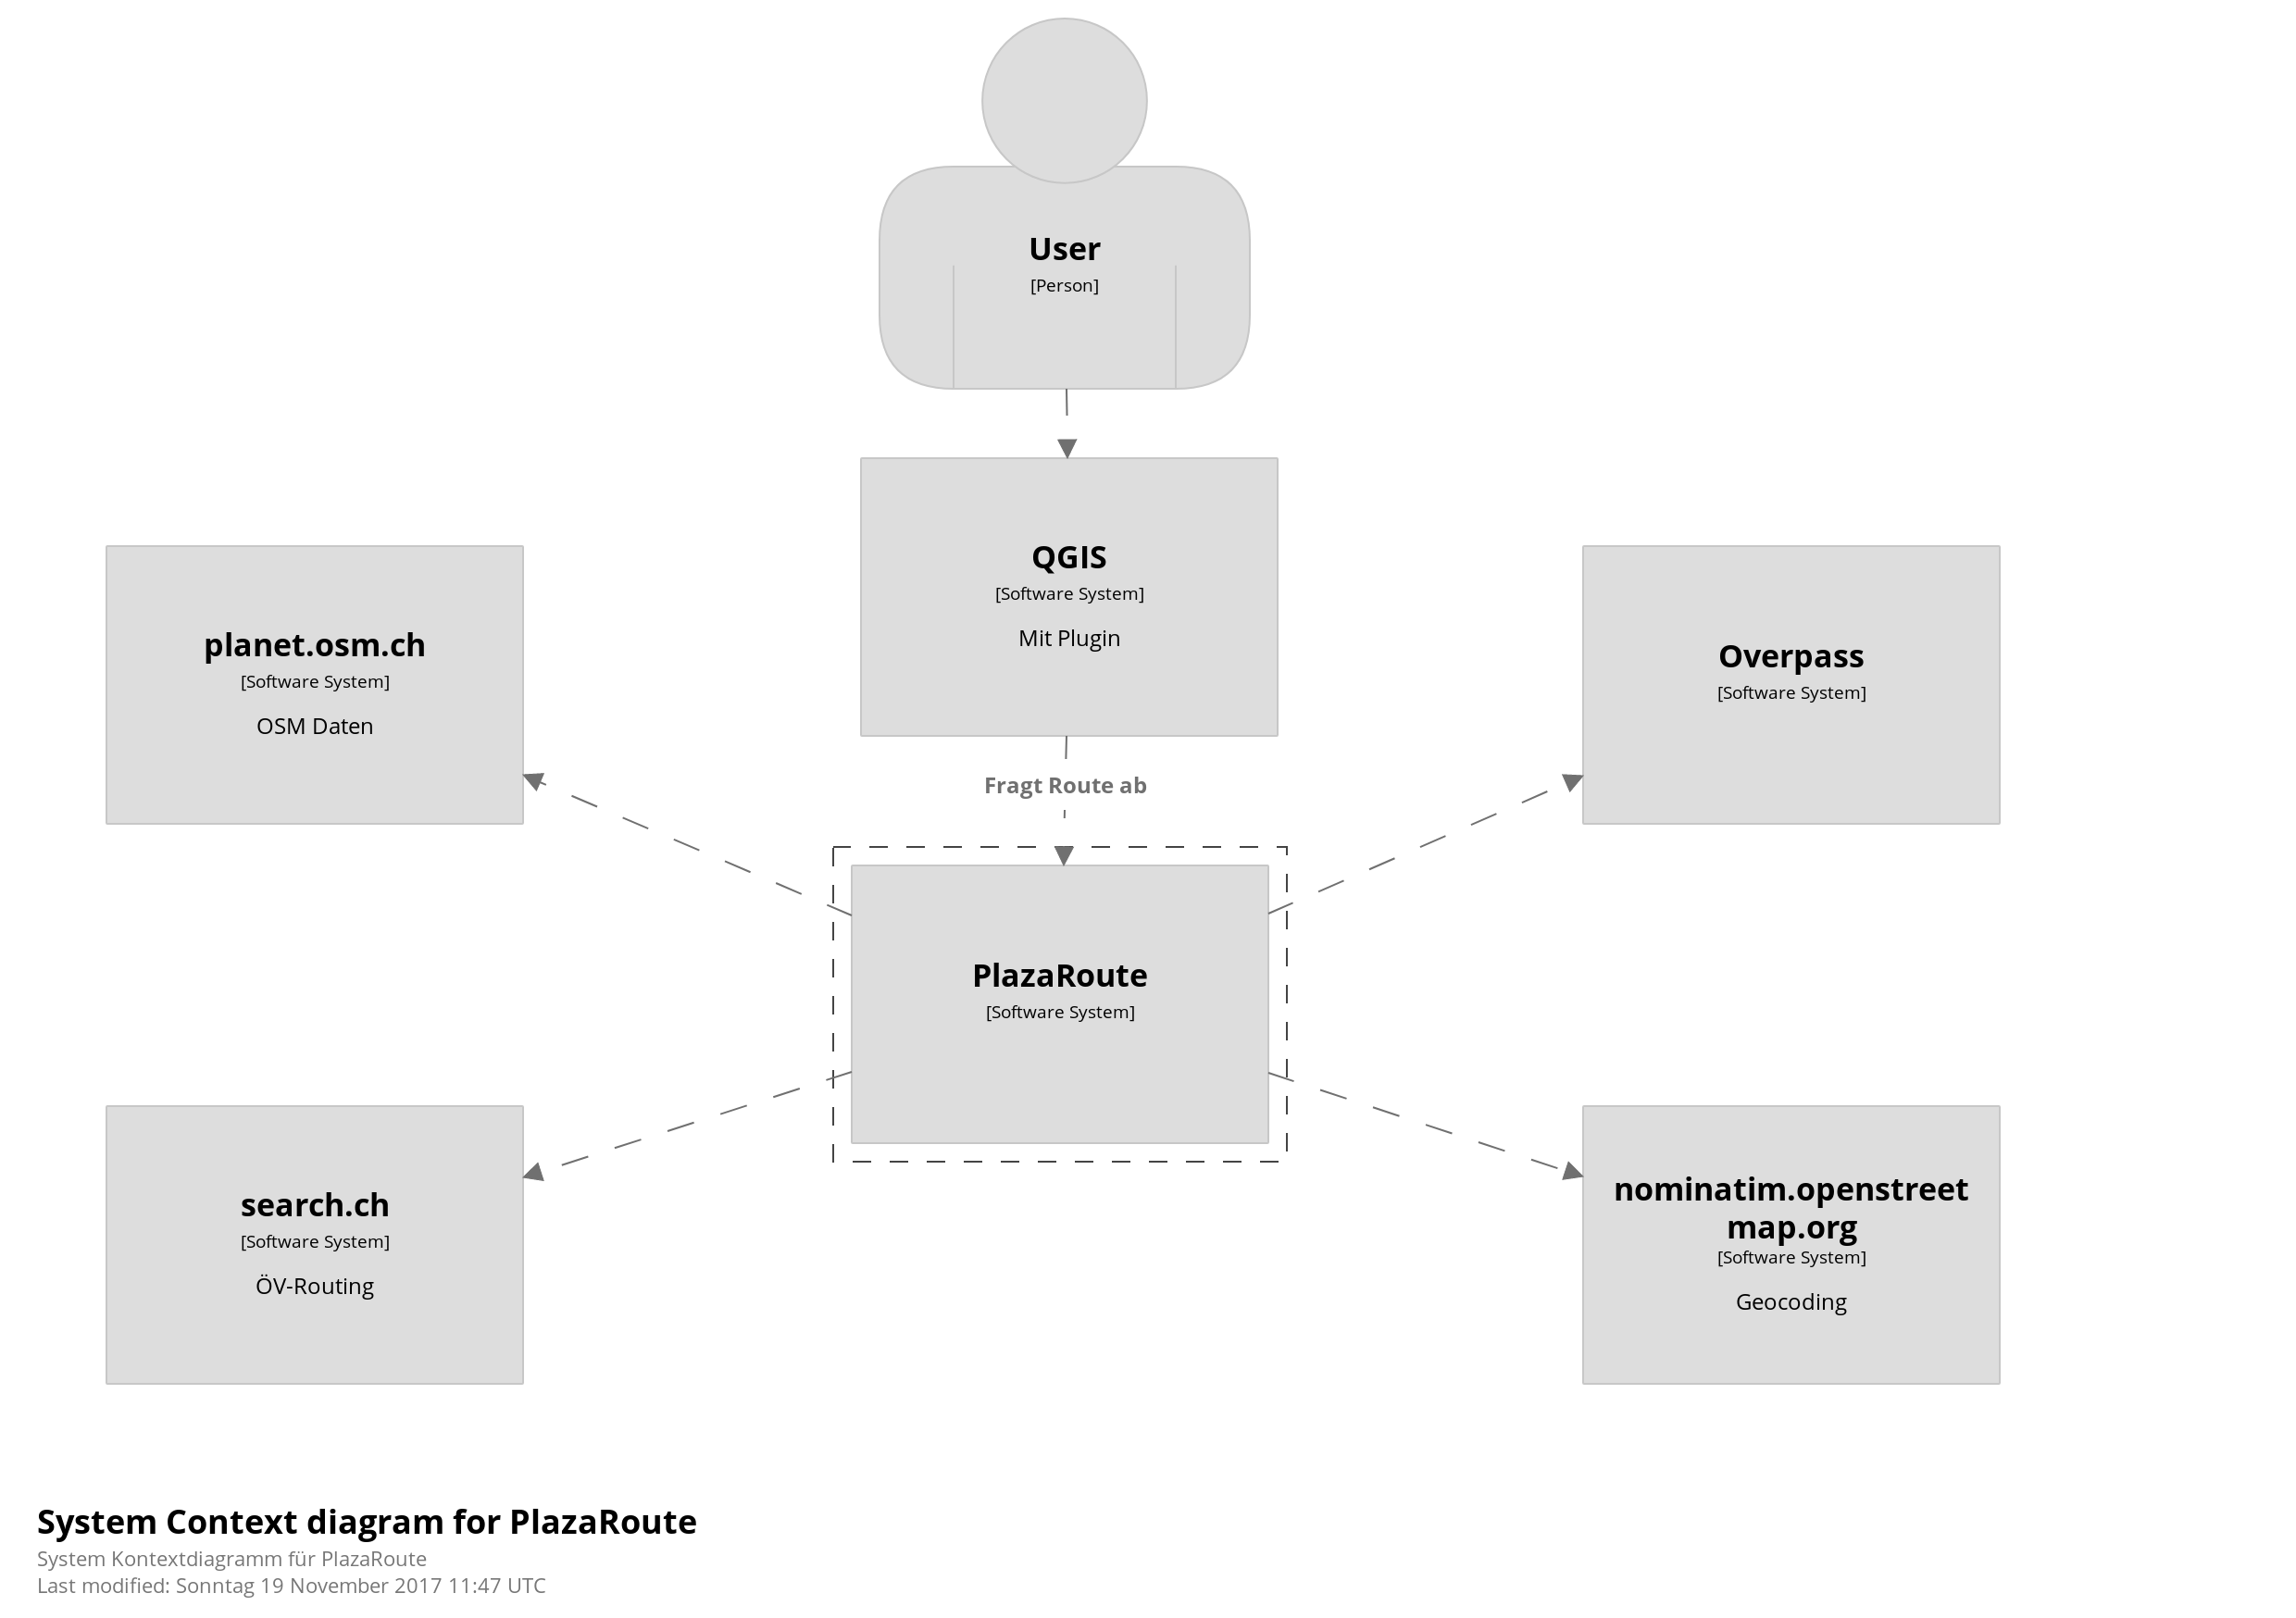
\includegraphics[width=1\linewidth]{projectdoc/img/system-context_diagram.png}
\caption[System Kontext Diagramm]{System PlazaRoute im Kontext mit Umsystemen; Grafik erstellt mit \emph{Structurizr Express}\cite{structurizr}}
\label{fig:system_context_diagram}
\end{figure}

Abbildung \ref{fig:system_context_diagram} zeigt das System PlazaRoute mit den Umsystemen auf. Beim Betrachten der C4-Diagramme ist zu beachten, dass diese nicht der \acs{UML}-Spezifikation folgen. Gestrichelte Pfeile bedeuten, dass eine Anfrage in Richtung der Pfeilspitze an ein System geht. Der Datenfluss läuft in die entgegengesetzte Richtung der Pfeile.

Der User bedient die QGIS Desktop Applikation mit dem von uns entwickelten Plugin. Dieses leitet die die Eingabe der Start- und Zielkoordinaten an das System PlazaRoute weiter. Als Antwort sendet PlazaRoute eine Routenbeschreibung an das QGIS-Plugin zurück, das es im QGIS darstellt.

\subsection{PlazaRoute Container}
\label{architektur:PlazaRoute Container}

\begin{figure}[ht]
    \centering
    % TODO: Grafik zuschneiden
    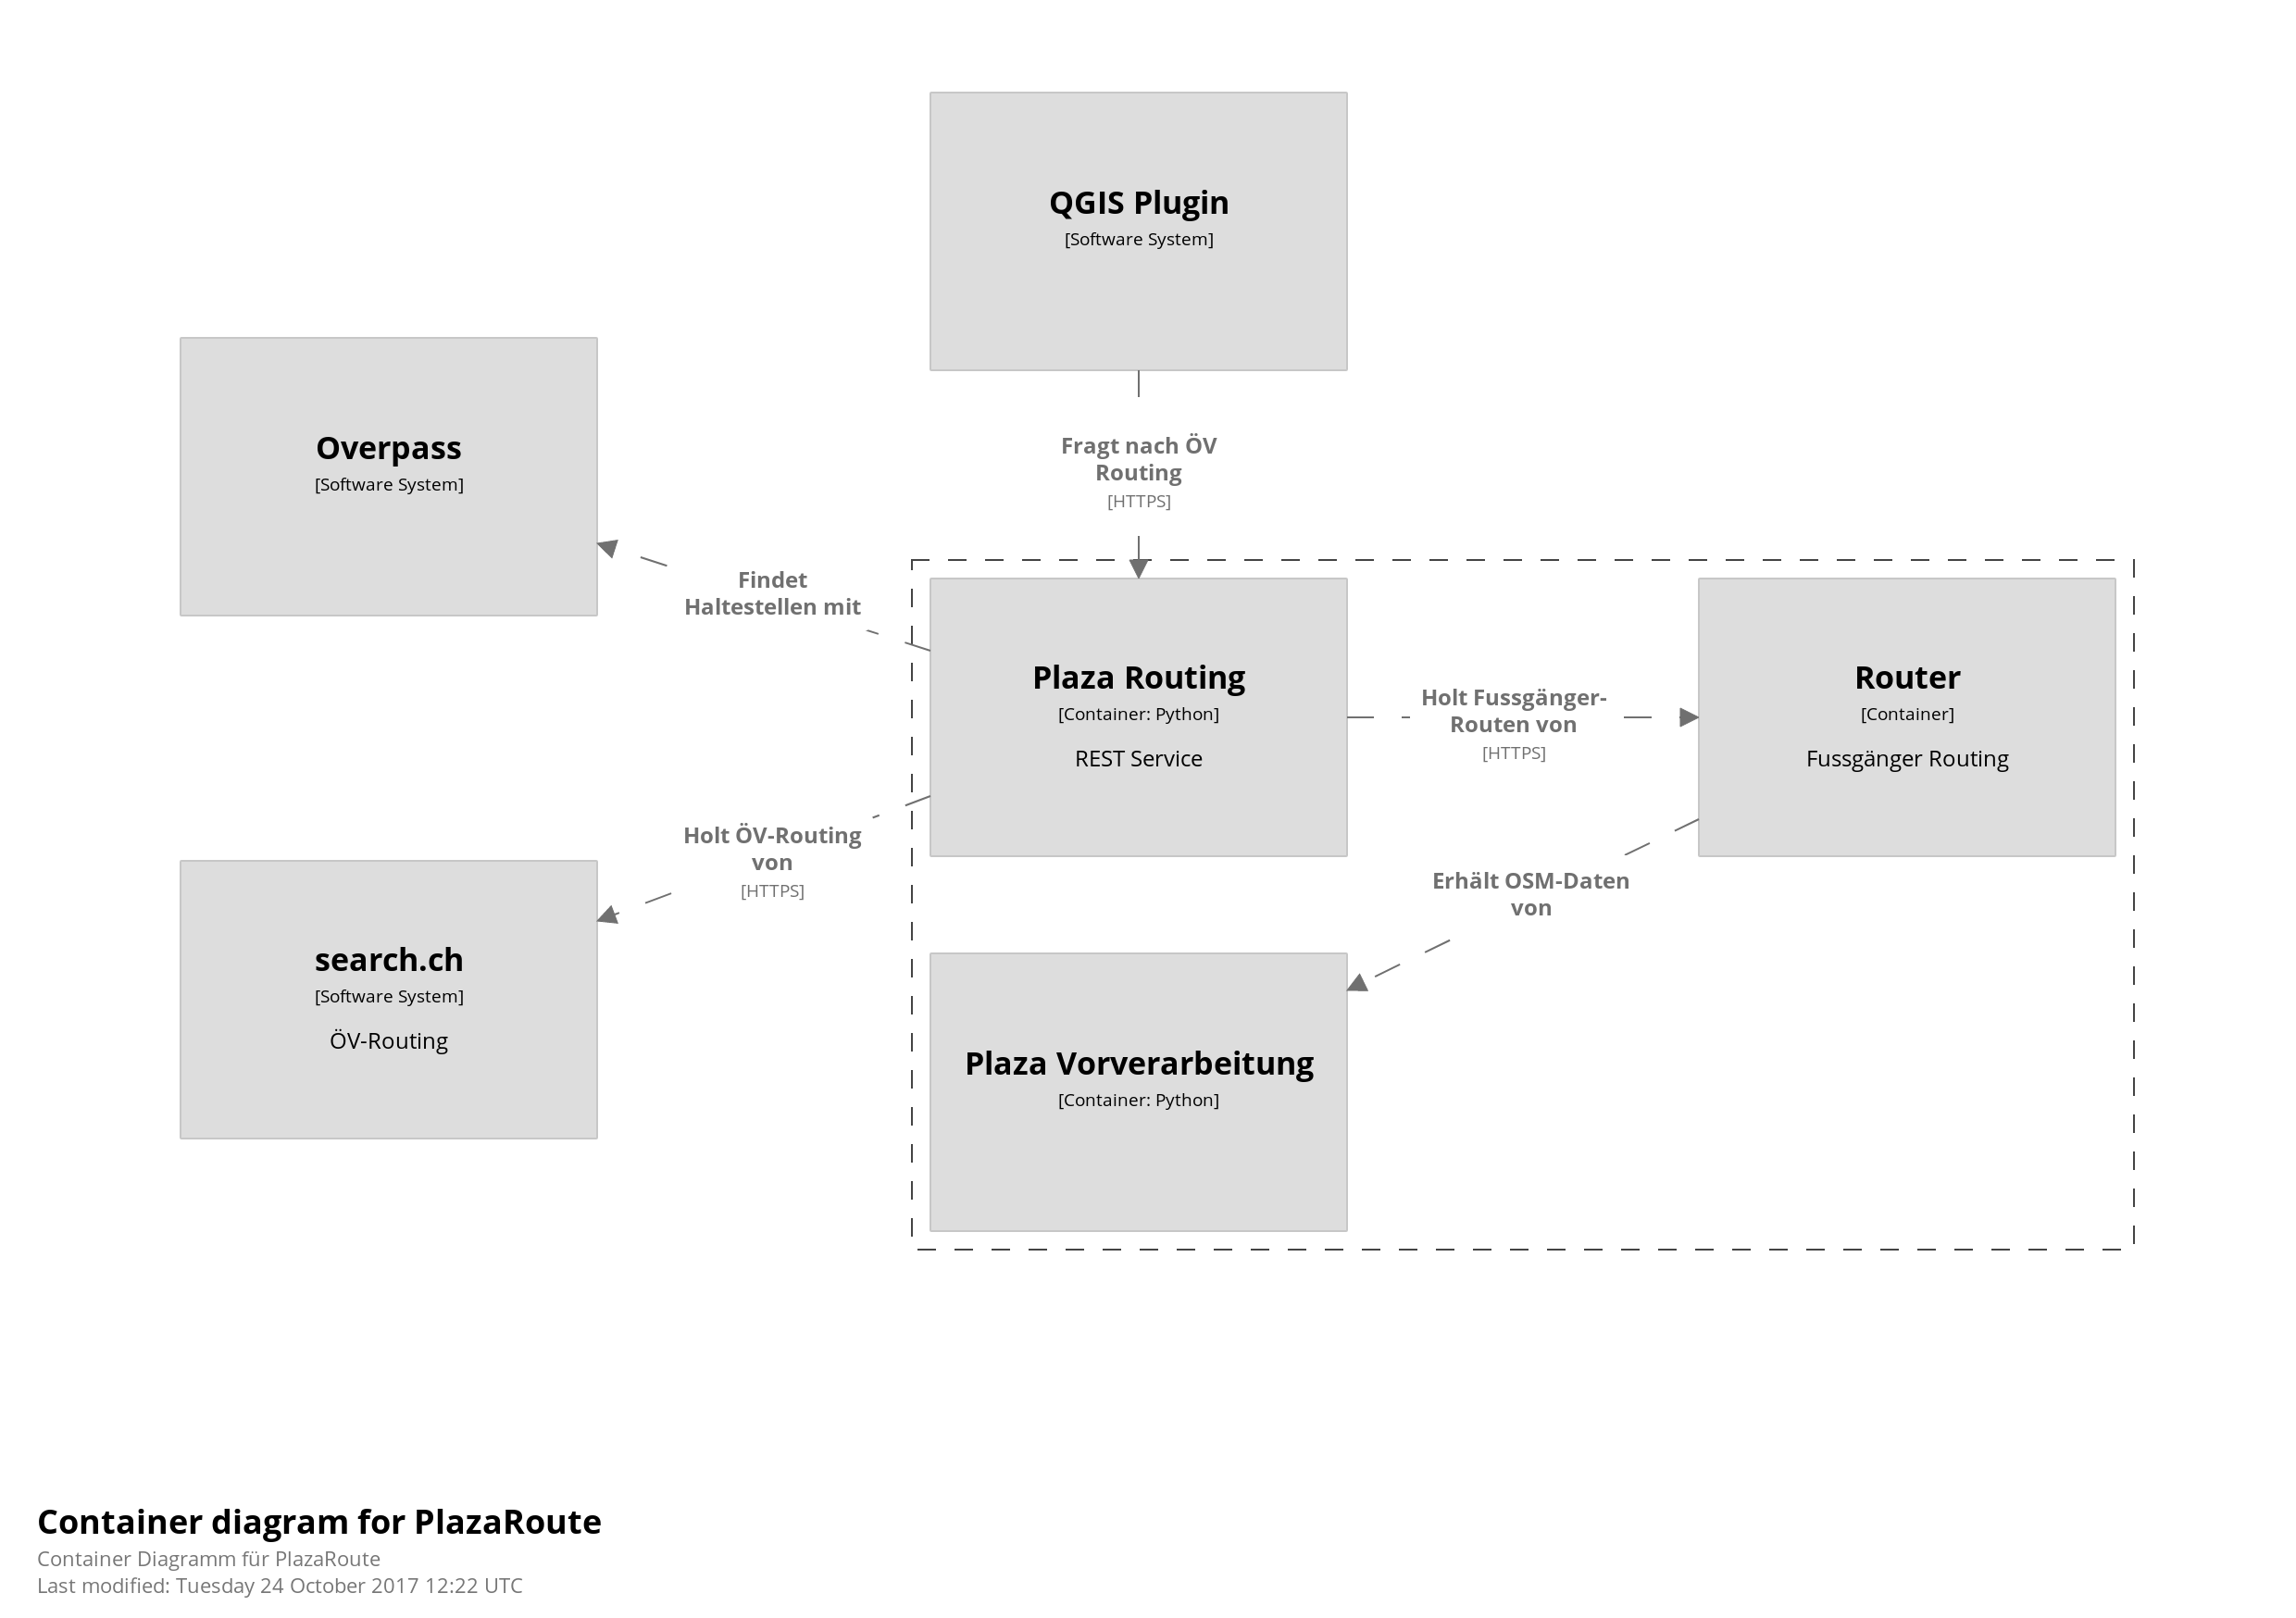
\includegraphics[width=1\linewidth]{projectdoc/img/container_diagram.png}
    \caption[Container Diagramm]{Container Diagramm von PlazaRoute; Das System PlazaRoute befindet sich in der eingerahmten Box; Grafik erstellt mit \emph{Structurizr Express}\cite{structurizr}}
    \label{fig:container_diagram}
    \end{figure}

In Abbildung \ref{fig:container_diagram} zoomen wir in das System PlazaRoute hinein und teilen es in drei Container auf, die logisch voneinander getrennt sind. So könnten die Container auch verteilt deployed werden.

In den nachfolgenden Abschnitten werden die drei Container näher beleuchtet.


\subsubsection{Plaza Vorverarbeitung}
\label{architektur:Plaza Vorverarbeitung}

Bevor die Routing Engine ihre Routing-Funktion ausführen kann, muss diese zuerst aus dem \ac{OSM}-Datensatz einen Routing-Graph generieren. Unsere Hauptaufgabe besteht darin, diesen Routing-Graphen für Fussgänger-Routing über Flächen zu optimieren. Ein Ansatz wäre, den Graphen nach dem Generieren zu verändern. Dies ist aber schwer realisierbar, da die meisten Routing-Engines die Graphen in eigenen (binären) Datenstrukturen ablegen. So wär unsere Implementation auch stark an eine einzelne Routing-Engine gekoppelt.

Ein zweiter Ansatz die Integration unserer Optimierung in die Verarbeitung der Routing-Engines selbst. Auch da wären wir wieder stark an eine spezifische Routing-Engine gekoppelt.
Wir haben uns stattdessen entschieden, beim Input der \ac{OSM}-Daten anzusetzen. Dazu werden die Rohdaten zuerst eingelesen und nach Fussgänger-Flächen abgesucht (\nameref{par:OSM Importer}). Mit unserem Algorithmus werden neue Fusswege eingetragen (\nameref{par:Plaza Optimizer}). Diese neu erzeugten Kartendaten werden dann wieder mit den ursprünglichen Rohdaten verschmelzt (\nameref{par:OSM Merger}). Erst dann generiert die Routing-Engine daraus den Routing-Graphen. Das Vorgehen ist in Abbildung \ref{fig:dataflow_vorverarbeitung} schematisch aufgezeigt.

Abbildung \ref{fig:component_diagram_vorverarbeitung} zeigt die einzelnen Komponenten für die Vorverarbeitung der \ac{OSM}-Daten auf. Darin werden die Komponenten des Containers Plaza Vorverarbeitung (siehe Abbildung \ref{fig:container_diagram}) in der gestrichelten Box dargestellt.


\begin{figure}[ht]
    \centering
    
\includegraphics[width=1\linewidth]{projectdoc/img/dataflow_vorverarbeitung.pdf}
    \caption[Datenfluss Vorverarbeitung]{Datenfluss-Diagramm der Vorverarbeitung von \ac{OSM}-Daten bis zur Übergabe an die Routing-Engine; Grafik erstellt mit \emph{draw.io}}
    \label{fig:dataflow_vorverarbeitung}
\end{figure}


\begin{figure}[ht]
\centering
% TODO: Grafik zuschneiden
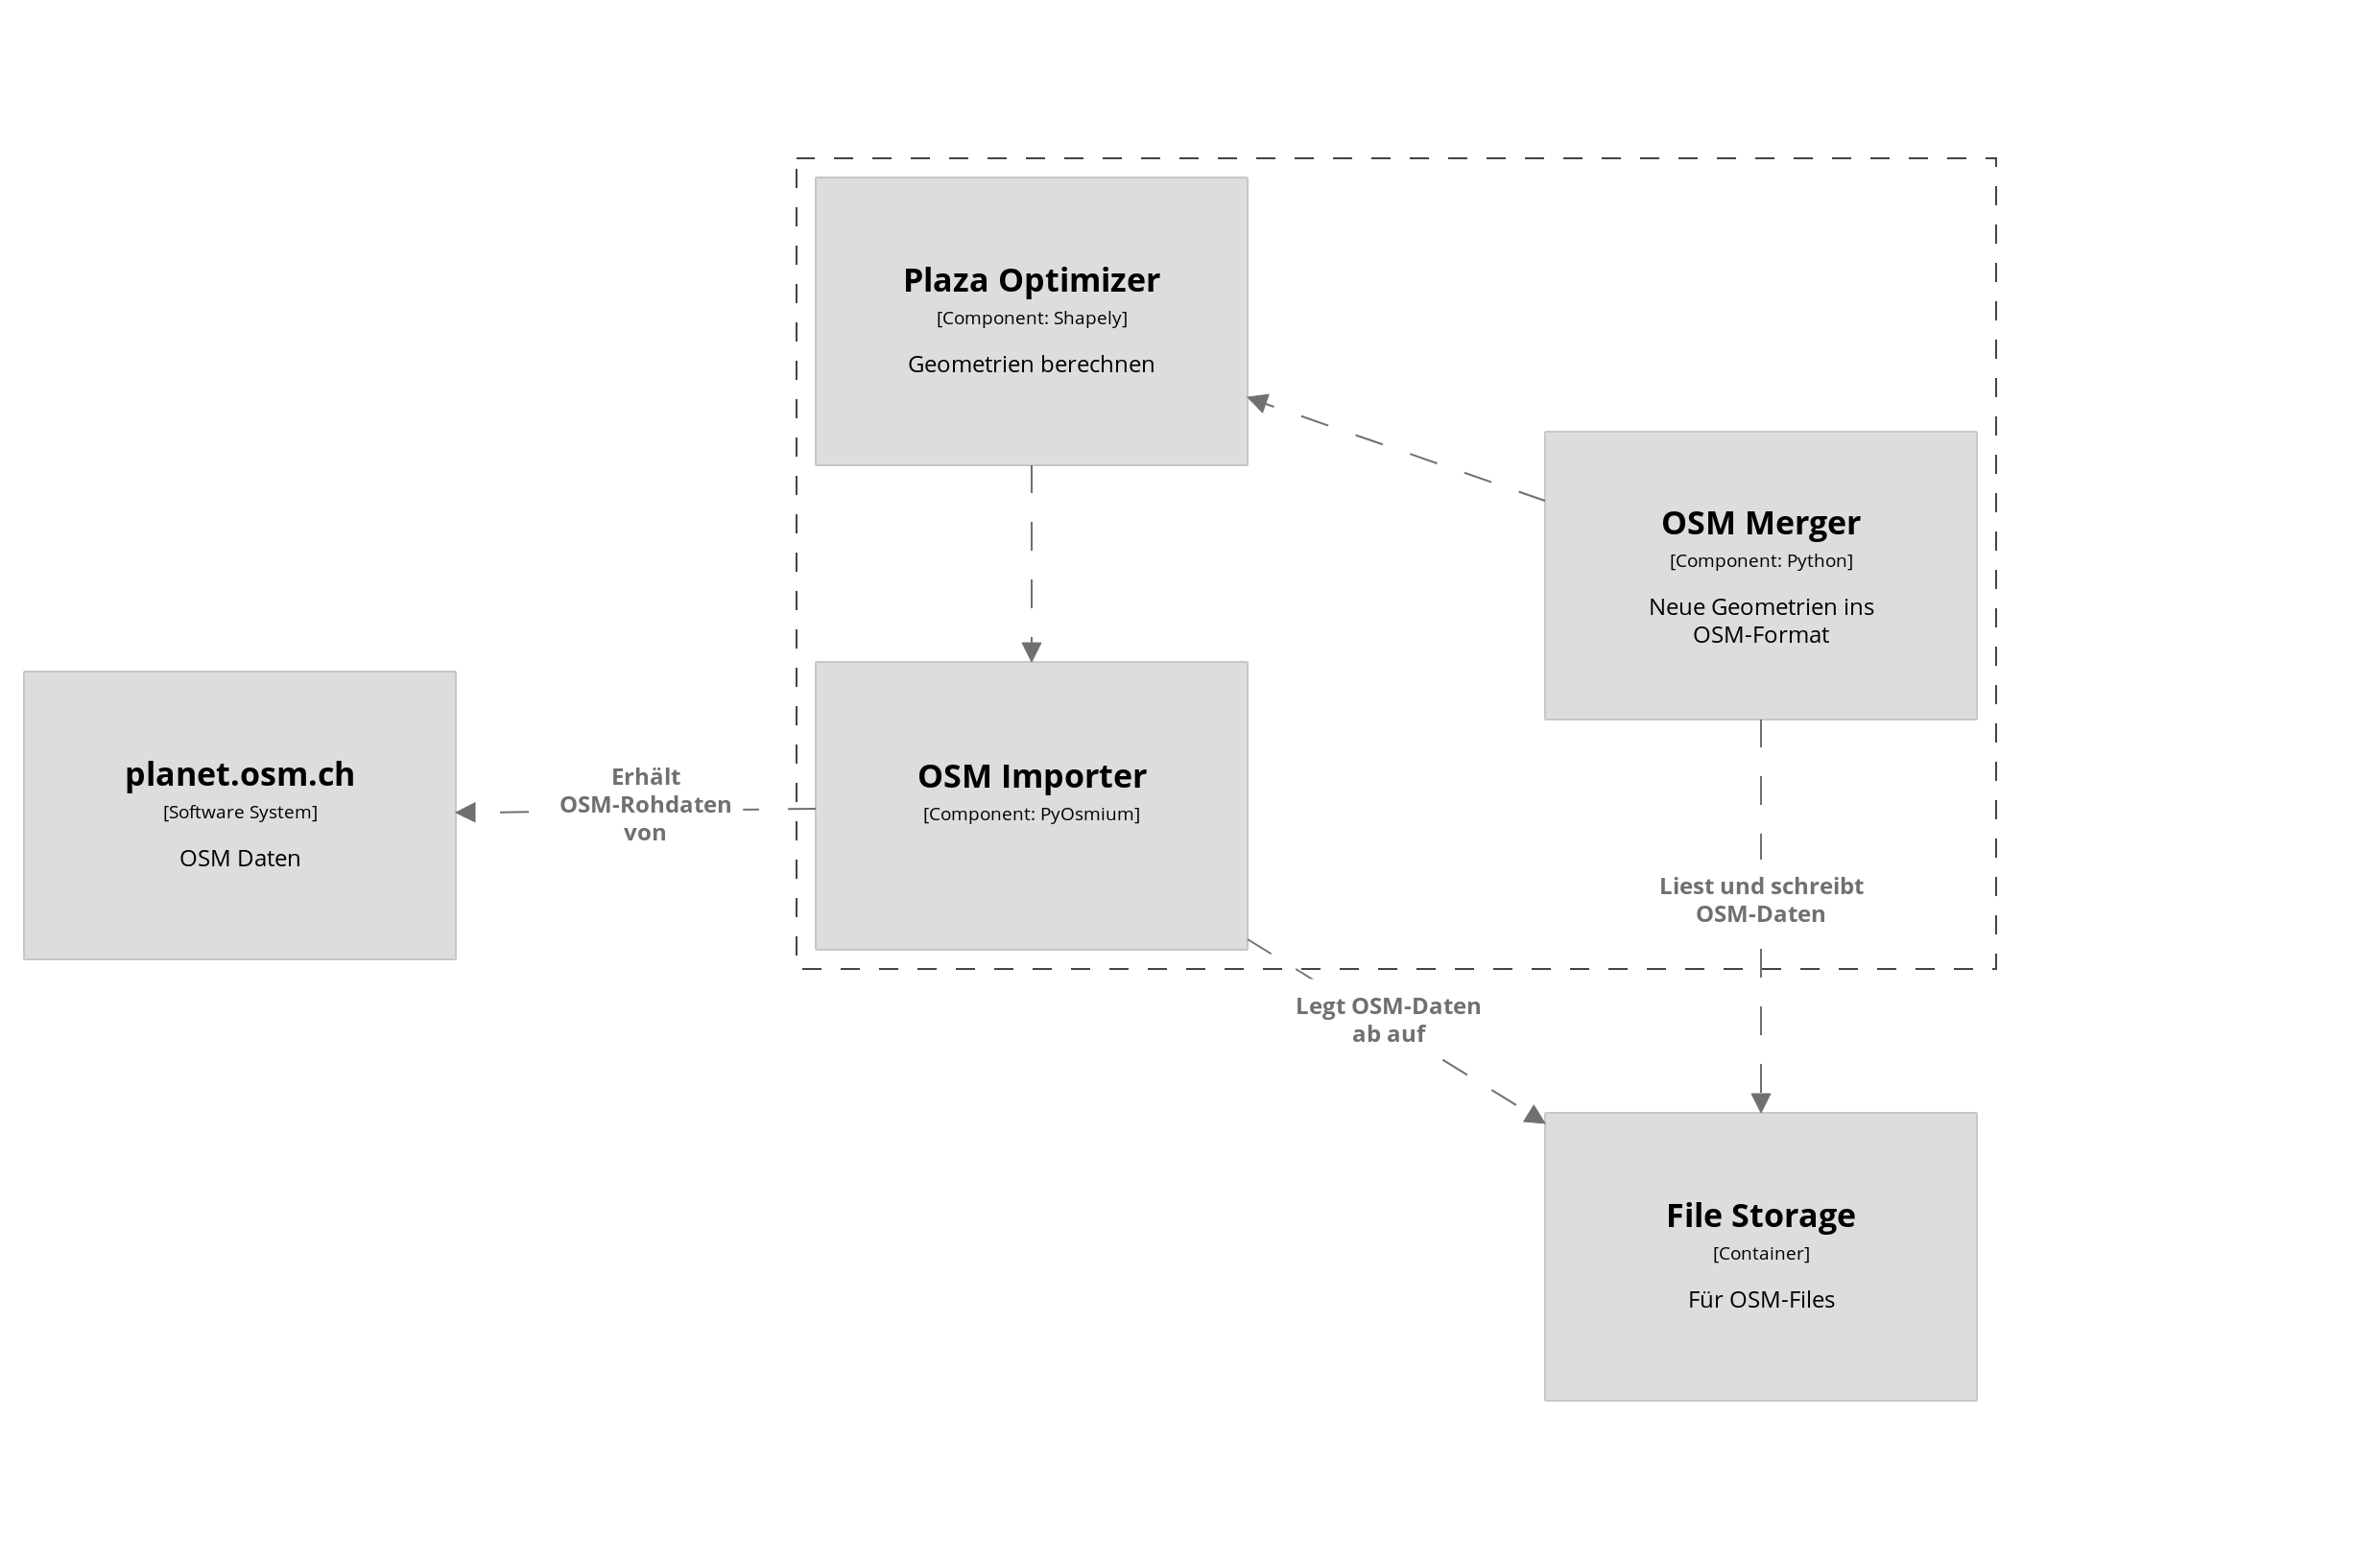
\includegraphics[width=1\linewidth]{projectdoc/img/component_diagram_plaza-vorverarbeitung.png}
\caption[Komponentendiagramm Vorverarbeitung]{Komponentendiagramm der Plaza Vorverarbeitung (eingerahmt); Grafik erstellt mit \emph{Structurizr Express}\cite{structurizr}}
\label{fig:component_diagram_vorverarbeitung}
\end{figure}


\paragraph{OSM Importer}\label{par:OSM Importer}~\\
Für unser optimiertes Routing wird in regelmässigen Abständen der neueste \ac{OSM}-Datensatz \cite{osm_data_switzerland} der Schweiz geladen. Die \acs{OSM}-Importer Komponente liest das komplette für uns relevante Kartenmaterial (z.B. die Schweiz) als \ac{PBF} ein und sucht dabei nach Flächen, die wir bearbeiten wollen.

Dazu werden \emph{Osmium} und die dazugehörigen Python-Bindings \emph{pyOsmium}\cite{pyosmium} verwendet. Osmium erkennt automatisch Flächen aus \ac{OSM} Multipolygone oder Relationen. Mit einem eigenen Handler können wir dabei gleich das Einlesen des Files auf die für uns interessanten Flächen beschränken, wie in Listing \ref{osmium_import_code} gezeigt wird.

%TODO: In Implementation verschieben?

\begin{listing}[ht]
    \inputminted{python}{projectdoc/listing/osmium_handler.py}
    \caption[Einlesen OSM-Daten mit Osmium]{Einlesen von OSM Daten mithilfe von \emph{Osmium}; Filterung auf für uns relevante Flächen}
    \label{osmium_import_code}
\end{listing}

\paragraph{Plaza Optimizer}\label{par:Plaza Optimizer}~\\
Die mit Osmium importierten \ac{OSM}-Daten sind noch reine \ac{OSM}-Objekte, auf denen keine Geometrie-Berechnungen angewendet werden können. Dazu wird die Python-Library \emph{Shapely}\cite{shapely} verwendet. Shapely kann mit Geometrien umgehen und Algorithmen von \ac{GEOS} wie \code{intersection} und \code{contains} darauf anwenden.

Um die mit Osmium importierten Objekte in Shapely zu verwenden, werden diese ins \ac{WKB} Format übersetzt und Shapely übergeben, wie in Listing \ref{shapely_import_code} gezeigt.

\begin{listing}[ht]
    \inputminted{python}{projectdoc/listing/shapely_import.py}
    \caption[Einlesen OSM Objekte in Shapely]{Übergabe von Osmium-Objekten zu Shapely für die Weiterverarbeitung}
    \label{shapely_import_code}
\end{listing}



\paragraph{OSM Merger}\label{par:OSM Merger}~\\
Der OSM Merger ist dafür verantwortlich, unsere erzeugten Geometrien (Fusswege) wieder in das \ac{OSM}-Kartenmaterial einzupflegen, um es anschliessend der Routing-Engine zur Verarbeitung zum Routing-Graphen zu übergeben.

Die durch unseren Algorithmus erzeugten Wege durch Flächen (in Shapely Datenstrukturen) sollen nun wieder zurück ins \ac{OSM}-Format geschrieben werden. Dazu wird wie beim \nameref{par:OSM Importer} Osmium verwendet, mit dem Geometrien in eine OSM-Datei geschrieben werden können

In einem weiteren Schritt müssen unsere optimierten Wege in das bestehende Strassennetz eingebunden werden, damit die Routing-Engine diese auch beachtet. Dazu werden die Eingangspunkte der von uns erzeugten Fusswege in den bestehenden Strassen und Wegen referenziert, die an diesem Punkt auf die Fläche treffen. Somit werden sie topologisch direkt miteinander verbunden.
% TODO: Begriff Eintrittspunkt definieren

Als letzten Schritt führen wir die erzeugten Fusswege und die modifizierten Strassen wieder zusammen mit der "grossen" \ac{OSM}-Datei, die ganz am Anfang importiert wurde. Dazu wird das Commandline-Tool Osmosis \cite{osmosis} verwendet.

\subsubsection{Plaza Routing}
\label{architektur:Plaza Routing}
Der Plaza Routing Container (siehe Abbildung \ref{fig:container_diagram}) ist für das Koordinieren und Verarbeiten von Routing-Anfragen verantwortlich. Er bietet für das QGIS-Plugin eine API an. Mit Hilfe von verschiedenen Drittsystemen und der Routing-Engine (für Fussgänger-Routing) wird eine komplette Route mit Fahrplan erstellt und dem QGIS-Plugin oder anderen Konsumenten übergeben.

In diesem Abschnitt wird vertieft in die einzelne Bestandteile des Plaza Routing eingegangen. So sind nachfolgend die einzelnen Schichten und Konstrukte aufgeführt und beschrieben. Zur Übersicht findet man das Schichten-Diagramm in Abbildung \ref{fig:package_diagram_plaza_routing}. Die Verantwortlichkeiten der Drittsystemen wird in den jeweiligen Schichten angesprochen.

\begin{figure}[ht]
\centering
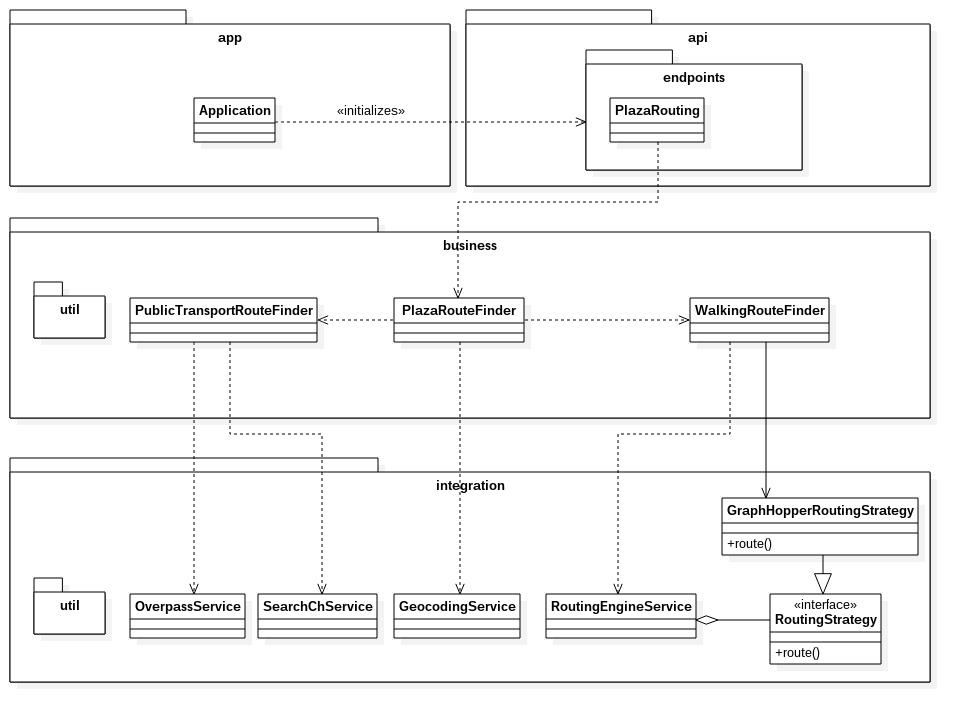
\includegraphics[width=1\linewidth]{projectdoc/img/package_diagram}
\caption[Schichten-Diagramm Plaza Routing]{Schichten-Diagramm Plaza Routing}
\label{fig:package_diagram_plaza_routing}
\end{figure}

\paragraph{app}\label{architektur:app-layer}~\\
Hierbei handelt es sich um den zentralen Einstiegspunkt in die Komponente \emph{PlazaRouting}. Die Komponenten wird in dieser Schicht konfiguriert und initialisiert.

\paragraph{api}\label{architektur:api-layer}~\\
In dieser Schicht wird eine \ac{REST}-\ac{API} für den gesamten externen Einstieg in das Plaza Routing exponiert. Diese \ac{API} wird primär vom \nameref{architektur:QGIS Plugin} verwendet. Eine Einschränkung bezüglich der Konsumenten gibt es nicht.

Die \ac{OAS} \cite{open-api-specificaiton} der \ac{API} ist unter \cite{plaza-routing-api-spez} verfügbar. SwaggerUI kann unter \cite{plaza-routing-api-swaggerui} eingesehen werden. Die {API}-Spezifikation wird in einem Git-Repository gehalten. Änderungen werden somit automatisch auf der Github-Page \cite{plaza-routing-api-spez} publiziert. Dies hat die Vorteile, dass es keine Abweichung zwischen Spezifikation und Dokumentation geben kann, mit Swagger \cite{swagger} die Schnittstelle bereits ideal beschrieben ist und die Haltung in einem öffentlichen Repository eine Diskussions-Plattform für Konsumenten bietet.

\paragraph{business}\label{architektur:business-layer}~\\
In der Business-Schicht ist die Business-Logik der \ac{API}-Abfragen vorhanden. Das PlazaRouting wird logisch in zwei Bereiche \emph{PublicTransportConnectionFinder} und \emph{WalkingRouteFinder} aufgeteilt. Die Koordination übernimmt dabei \emph{PlazaRouteFinder}. So wird das Design-Prinzip \emph{Separation of Concern} ideal umgesetzt, da \emph{PublicTransportConnectionFinder} nur mit Services kommuniziert, welche für das ÖV-Routing notwendig sind und \emph{WalkingRouteFinder} die Kommunikation mit der Routing-Engine übernimmt.

\paragraph{integration}\label{architektur:integration-layer}~\\
In den nachfolgenden Abschnitten sind die Integration-Services und ihre Notwendigkeit beschrieben. In dieser Architektur werden Komponenten, welche mit Drittsystemen oder -komponenten kommunizieren als \emph{Services} bezeichnet und der Integration-Schicht angegliedert.

\subparagraph{Search.ch Service}\label{architektur:Search.ch Service}~\\
Der \emph{SearchChService} kommuniziert mit der Fahrplan-\ac{API} von search.ch \cite{search_ch_route_api} und bezieht die Fahrplan-Daten für eine bestimmte Ausgangsstation und Destination.

\subparagraph{Overpass Service}\label{architektur:Overpass Service}~\\
Der \emph{OverpassService} übernimmt mithilfe der \ac{QL} die Kommunikation mit Overpass \cite{wiki:overpass}. Der Hauptfokus liegt auf dem Extrahieren von ÖV-Stationen in einem gegebenen Umkreis und geografischen Position von ÖV-Stationen basierend auf Daten, welche aus dem \nameref{architektur:Search.ch Service} gewonnen werden.

\subparagraph{Geocoding Service}\label{architektur:Geocoding Service}~\\
Der \emph{GeocodingService} liefert für eine Adresse eine Koordinate.

\subparagraph{Routing-Engine Service}\label{architektur:Routing-Engine Service}~\\
Der \emph{RoutingEngineService} ist für das Fussgänger-Routing zuständig und kommuniziert mit einer Routing-Engine. Die Architektur ist mit dem Strategy-Pattern \cite{gof_patterns} so gewählt, dass die Routing-Engine einfach ausgetauscht werden kann.

\subsection{QGIS Plugin}
\label{architektur:QGIS Plugin}

Das QGIS-Plugin ist unabhängig vom System PlazaRoute und läuft auf dem Client des Benutzers. Die Kommunikation mit dem Container Plaza Routing erfolgt über einen REST-Service. Das Plugin ist reiner Konsument und zeigt auf, welchen Mehrwert PlazaRoute bieten kann. In Abbildung \ref{fig:class_diagram_plaza_route_qgis_plugin} ist das Klassen-Diagramm zu sehen. Herausheben kann man, dass das Plugin in fünf Komponente zerlegt wird. \emph{PlazaRouteRoutingService} kommuniziert mit dem REST-Service (siehe Abschnitt \nameref{architektur:api-layer}). \emph{PlazaRouteMapTool} übernimmt die Interaktion mit der Karte und führt das Zeichnen der Route mit \emph{PlazaRouteRouteDrawer} durch. \emph{PlazaRouteDirectionsGenerator} generiert ein Routing für die zurückgelieferte Route. Die zentrale Steuerung übernimmt das Dockwidget.

\begin{figure}[th]
\centering
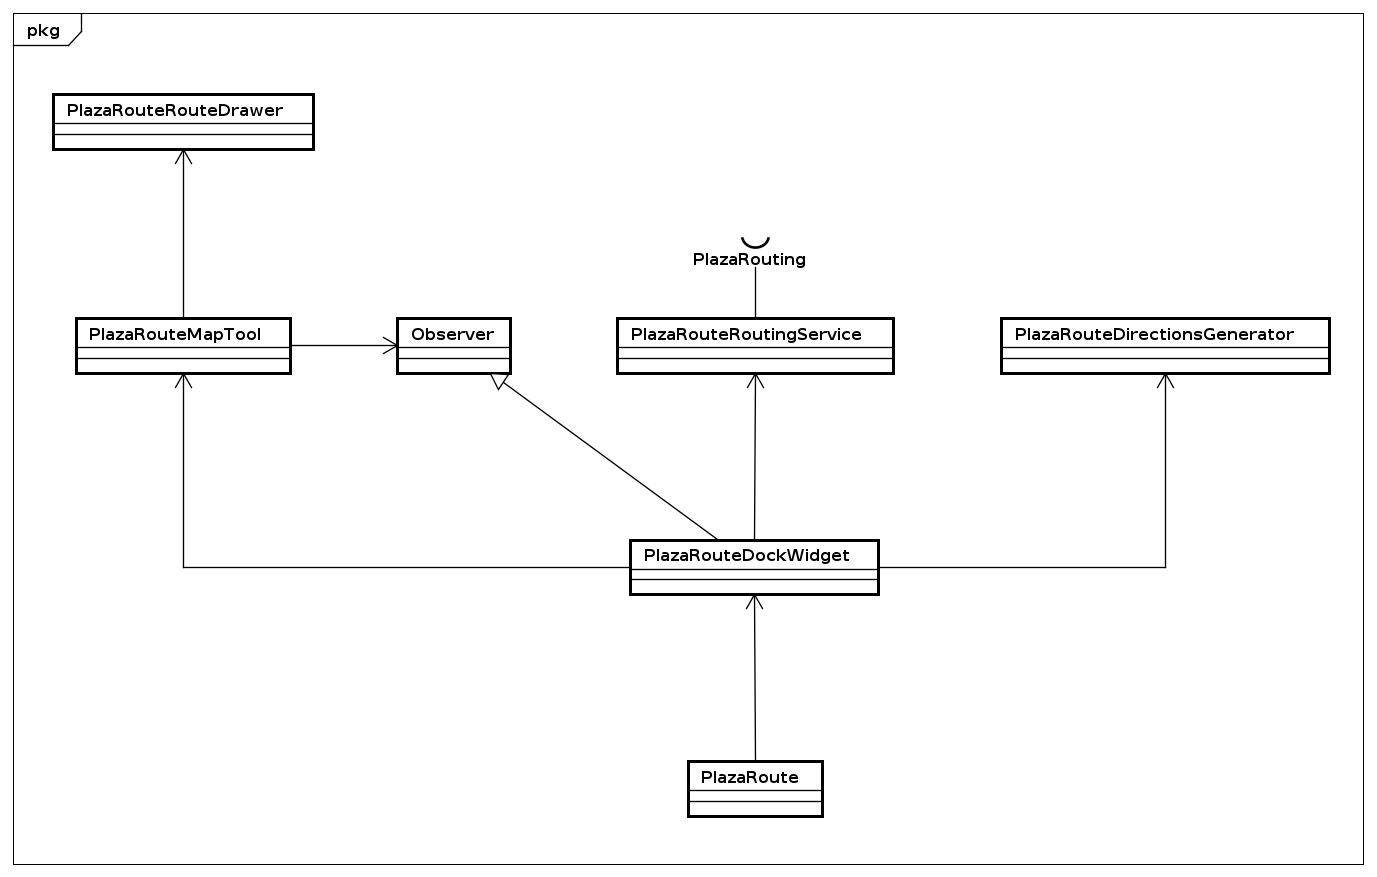
\includegraphics[width=1.0\linewidth]{projectdoc/img/class_diagram_plaza_route_qgis_plugin}
\caption[Klassen-Diagramm Plaza Route QGIS Plugin]{Klassen-Diagramm Plaza Route QGIS Plugin}
\label{fig:class_diagram_plaza_route_qgis_plugin}
\end{figure}



\section{Implementation}
\label{sec:Implementation}

\subsubsection{Komponenten}
\label{subsub:impl_Komponenten}


\section{Tests}
\label{sec:Tests}
% Manuelle und automatische Tests

\subsection{Strategie}
\label{test:Strategie}
Grundsätzliches Ziel war es, beim Entdecken von Grenzfällen und Fehlern nach dem \ac{TDD}-Zyklus vorzugehen. Für das Testing wurden Unit- und Integration-Tests grosszügig eingesetzt. Durch die Gegebenheiten der Problem-Domäne ist es von besonderer Wichtigkeit, dass möglichst breit und viel getestet wird. Dadurch kann den Problemen, welche durch ein "fehlendes" \ac{OSM}-Datenmodell auftreten, entgegen gewirkt werden.  Die Tests werden automatisiert bei jedem Commit mit Continuous Integration durch CircleCI \cite{circleci} ausgeführt. So ist sichergestellt, dass Builds, welche auf einem Feature-Branch fehlschlagen, nicht in den Master gemerged werden. Im nachfolgenden sind die Tests für die Komponenten \emph{Plaza Vorverarbeitung} und \emph{Plaza Routing} getrennt aufgeschlüsselt, da die Applikationen mit unterschiedlichen Bedingungen zu kämpfen haben.


\subsection{Plaza Vorverarbeitung}
\label{test:Plaza Vorverarbeitung}
Bei \emph{Plaza Vorverarbeitung} liegt der Fokus auf dem korrekten Zusammenspiel der Komponenten. Die Abbildung \ref{fig:dataflow_vorverarbeitung} zeigt dessen Datenfluss auf. Aus diesem Grund haben wir den Fokus auf Integration-Tests gelegt. So wird unter anderem beim Testen des \nameref{impl:Optimizer} auch der \nameref{impl:Importer} verwendet, da das Mocken der internen in-memory Datenstruktur, welche der \nameref{impl:Importer} liefert, keinen Sinn macht, da dieser aufgrund der vordefinierten \ac{OSM}-Dateien deterministische Daten liefert. In Fällen wo diese Annahme nicht zutrifft und Funktionen in Isolation getestet werden können, werden Unit-Tests, wie in Listing \ref{Unit-Test Shortest-Path} sichtbar, eingesetzt.

\begin{listing}[ht]
    \inputminted{python}{projectdoc/listing/test_compute_dijkstra_shortest_paths.py}
    \caption{Unit-Test Shortest Path}
    \label{Unit-Test Shortest-Path}
\end{listing}

In Listing \ref{Integration-Test Plaza Preprocessor} ist aufgeführt, wie das Unit-Testing gehandhabt wird. Durch Fixtures kann der Tests in diesem Fall auf vier verschiedene Arten von möglichen Konfigurationen getestet werden, beispielsweise eine Visibility-Graph Vorverarbeitung, welche den A* \cite{astar} als \gls{Shortest-Path}-Algorithmus verwendet.

\begin{listing}[ht]
    \inputminted{python}{projectdoc/listing/test_plaza_prepreprocessor.py}
    \caption{Integration-Test Plaza Preprocessor}
    \label{Integration-Test Plaza Preprocessor}
\end{listing}

\subsection{Plaza Routing}
\label{test:Plaza Routing}

\emph{Plaza Routing} verwendet Fremdsysteme für unterschiedliche Zwecke. Unter anderem wird search.ch \cite{search_ch_route_api} für das Abfragen der ÖV-Verbindungen benötigt. Werden nun Tests direkt auf dem Fremdsystem durchgeführt, kann man nicht mit einem deterministischen Verhalten rechnen. Die Werte sind in diesem konkreten Fall datumsabhängig. So werden beispielsweise am Sonntag nicht die gleichen Verbindungen angeboten wie unter der Woche. Auch die Abfrage auf ein konkretes Datum ist nur beschränkt möglich, da die Daten nur einen gewissen Zeitraum in die Vergangenheit abrufbar sind. Bei Overpass \cite{wiki:overpass} liegt die Problematik bei den zugrundeliegenden Daten. Es liegt in der Natur der \ac{OSM}-Daten, dass sie sich stetig verändern. Stabile Tests sind in diesem Fall nicht möglich, wenn man wie in Kap. \ref{impl:Plaza Routing Route optimieren} von Koordinaten abhängig ist und diese direkt auf dem Fremdsystem überprüfen will. Diese Erfahrung wurde im Verlauf des Projekts gemacht. So wurden nachträglich Mocks eingeführt, welche stabile Tests ermöglichen. In Listing \ref{Mock search.ch} ist zu sehen, wie mit \emph{monkeypatch} \cite{pytest} für search.ch \cite{search_ch_route_api} aufgrund der übergebenen Parameter die erwartete Antwort geliefert wird. 

\begin{listing}[ht]
    \inputminted{python}{projectdoc/listing/mock_search_ch.py}
    \caption{Mock search.ch}
    \label{Mock search.ch}
\end{listing}

Durch diesen Ansatz lassen sich Unit- und Integration-Tests auf einer stabilen Datenbasis durchführen.

\subsubsection{Healthchecks}
\label{test:Healthchecks}
Da alle Services in den Tests gemockt werden, ist es unabdingbar, dass mit Healthchecks die Fremdsysteme geprüft werden. So ist sichergestellt, dass der Aufruf auf das konkreten System mit den bewährten Parameter eine erfolgreiche Rückmeldung liefert und das Fremdsystem verfügbar ist. Ob die Werte ansatzweise sinnvoll sind, wird durch die jeweiligen Parser der Services sichergestellt.

\subsection{Fazit}
\label{test:Fazit}

\subsubsection{TDD}
\label{fazit:TDD}
Das Vorgehen nach dem \ac{TDD}-Zyklus hat sich vor allem beim Arbeiten mit Fremdsystemen extrem bewährt. Herauszuheben ist hier das Optimieren von Routen, welches im Abschnitt \nameref{impl:Plaza Routing Route optimieren} behandelt wurde. Hier wurde intensiv mit Overpass \cite{wiki:overpass} kommuniziert. Durch die Gegebenheit der \ac{OSM}-Daten und den Freiheiten der Mapper sind Grenzfälle und unerwartete Abbildungen der Daten keine Seltenheit. In diesen Fällen hat man Tests erstellt, welche das Verhalten reproduzieren und auf das zu Erwartende prüfen und konnte so die Logik modifizieren, damit das wie im Implementationskapitel beschriebene fehlertolerante System umgesetzt werden konnte.

\subsubsection{Tests mit Fremdsystemen}
\label{fazit:Tests mit Fremdsystemen}
Beim Arbeiten mit den Fremdsystemen hat sich gezeigt, dass es sich lohnt, die Resultate der Service-Aufrufe von Anfang an zu mocken, wenn man im Vorhinein bereits weiss, dass die zugrundeliegende Daten transient sind. Der Aufwand ist in diesem Fall nicht zu unterschätzen, hat sich aber in unserem Fall definitiv gelohnt.

\subsubsection{Python Typensystem}
\label{fazit:Python Typesystem}
Vorallem bei einer Sprache mit einem dynamischen Typensystem wie bei Python ist es wichtig, dass ausgiebig getestet wird. Ändert sich beispielsweise die Struktur eines Rückgabewerts, sind die Auswirkungen dieser Änderungen nicht sofort sichtbar. Wird diese Stelle jedoch zusätzlich getestet, ist jederzeit klar, ob es sich um Breaking-Changes handelt. Mit den in Python 3 eingeführten "Type Hints" konnte dieses Problem aber schon etwas eingedämmt werden.


\section{Resultate und Weiterentwicklung}
\label{sec:Resultate und Weiterentwicklung}
% Resultate und Ergebnisse der Arbeit. Dieser Abschnitt richtet sich an den speziell für das entsprechende Fachgebiet interessierten Ingenieur. Er soll es ihm ermöglichen, die für die Problemlösung gemachten Überlegungen zu verstehen und nachzuvollziehen.

\subsection{Resultate}
\label{sub:Resultate}

Mit unserer Implementation der Algorithmen zur Flächen-Traversierung kann gezeigt werden, wie ein natürlicheres Routing für Fussgänger, insbesondere über offene Flächen, erreicht werden kann. Mit dem PlazaRouting Backend wurde dabei eine praktische Anwendung umgesetzt, die das Routing mit öffentlichen Transportmitteln zusammen mit optimiertem Fussgänger-Routing ermöglicht. Insbesondere haben wir Ansätze gezeigt, wie für Haltestellen genaue Koordinaten berechnet werden können (Kap. \ref{impl:Plaza Routing Route optimieren}). Die Routen können mit dem QGIS-Plugin berechnet und visualisiert werden.

\subsection{Möglichkeiten der Weiterentwicklung}
\label{sub:Möglichkeiten der Weiterentwicklung}


\subsubsection{Plaza Vorverarbeitung}
\label{subsub:Weiterentwicklung_Vorverarbeitung}

In Zukunft könnte unsere Implementation der Vorverarbeitung dazu dienen, die Optimierung auf Fussgänger-Routing in die Graphen-Berechnung von bestehenden Routing-Engines einzubinden. Somit würde der sepparate Schritt der Vorverarbeitung von \ac{OSM}-Daten entfallen, was durch den ersparten Aufwand des Lesens und Schreibens von \ac{OSM}-Daten die Effizienz deutlich steigern würde.

In der jetzigen Implementation werden die kürzesten Wege nur zwischen Paaren von \glspl{Einstiegspunkt}n berechnet. Dies hat zur Folge, dass auf einer Fläche mindestens zwei Einstiegspunkte vorhanden sein müssen, um Pfade berechnen zu können. Es gibt aber einige Fussgänger-Flächen, wo keine Strasse oder Weg den Platz angrenzt oder schneidet, wodurch keine Einstiegspunkte gefunden werden. In der Realität wäre der Platz aber mit grosser Wahrscheinlichkeit problemlos begehbar. Eine mögliche Lösung ist in Kap. \ref{subsub:Verbesserung_Einstiegspunkte} beschrieben.

Während der Entwicklung sind noch folgende Ideen und Ansätze aufgekommen:

\begin{itemize}
    \item Wenn zwei Fussgänger-Flächen direkt aneinander angrenzen, sollte dies für die Verarbeitung berücksichtigt werden. Lösungsansätze dazu sind in Kap. \ref{subsub:Routing bei zwei benachbarten Flächen} beschrieben.
    \item In der jetzigen Implementation wird die meiste Rechenzeit verwendet, um die \ac{OSM}-Daten für die Vorverarbeitung zu importieren. Es würde sich anbieten, die Daten in einer sepparaten Datenstruktur, z.B. PostGIS, zu halten, damit der Import-Schritt effizienter wird.
    \item Die Verarbeitung der einzelnen Flächen sind grundsätzlich unabhängig voneinander. So würde es sich anbieten, die Vorverarbeitung zu parallelisieren, um Multi-Core Systeme effizienter ausnutzen zu können.
    \item Python eignet sich gut als Sprache für den Prototypen. Für eine performante Verarbeitung würde sich eine Implementation mit einer Sprache wie C++ allerdings besser eignen. Es könnten auch nur Teile des Pythons-Code in C++ implementiert werden.
\end{itemize}

\subsubsection{Backend und QGIS-Plugin}
\label{subsub:Weiterentwicklung_Backend_QGIS}

Während der Entwicklung des PlazaRoute Services mit dem entsprechenden QGIS-Plugin sind folgende Verbesserungsmöglichkeiten aufgekommen:

\begin{itemize}
    \item Bei der Auswahl der optimalen ÖV-Route werden gewisse Annahmen getroffen über die Gewichtung von Laufwegen und die Wartezeit auf ÖV-Verbindungen. Benutzer haben allerdings unterschiedliche Präferenzen, ob sie lieber etwas länger laufen, anstatt auf eine Verbindung zu warten. Für diese Parameter könnten optimale Durchschnittswerte gefunden werden und es dem Benutzer ermöglichen, diese selbst zu konfigurieren.
    \item Vom Startpunkt aus wird in einem fixen Umfeld nach ÖV-Haltestellen gesucht. Pro gefundene ÖV-Haltestelle wird eine Route berechnet. Es wäre unter Umständen sinnvoller, die ÖV-Haltestellen in einem grösseren Umkreis zu suchen, aber nur ÖV-Verbindungen für die am nähesten liegenden ÖV-Haltestellen in Betracht zu ziehen.
    \item Bei ÖV-Verbindungen werden momentan nur die Koordinaten der Zwischenhaltestellen geliefert. In der Visualisierung werden zwischen diesen Koordinaten Geraden gezogen. Für eine genauere Darstellung ist es denkbar, ein separates Routing für ÖV-Verbindungen zu realisieren, das exakt den Strassen und Schienen des öffentlichen Verkehrsmittels folgt.
\end{itemize}

% Aufwandschätzung, Zeitplan, Projektplan
\section{Projektmanagement}
\label{sec:Projektmanagement}

\subsection{Vorgehen}
\label{sub:Vorgehen}

Für die Studienarbeit wurde das agile Vorgehen SCRUM in Kombination mit \ac{RUP} gewählt. Gründe für diese Entscheidung sind, dass das agile Vorgehen der noch zu Beginn offenen Aufgabenstellung entgegenkommt, welche dann iterativ finalisiert werden kann und dass die unbekannte Problem-Domäne sowie der theoretische Fokus der Arbeit so besser gehandhabt und schneller reagiert werden kann. Die wöchentlichen Besprechungen und Reviews mit dem Betreuer ist ein weiterer Grund für diese Entscheidung. Die Kombination mit \ac{RUP} ermöglicht es, dass Projekt in einzelne Phasen aufzuteilen, um so das Ziel und die Zeit nicht aus den Augen zu verlieren.

\subsubsection{Entwicklung}
\label{sub:Entwicklung}

Der Source-Code der Implementation wie auch diese Arbeit wird mit Git verwaltet und ist auf Github abgelegt. Die Entwicklung und das Dokumentieren erfolgt nach dem Github-Flow. Der Master-Branch ist auf allen Repositories während der ganzen Zeit gesperrt, so dass er nur über Pull-Requests bearbeitet werden kann. Für jede User-Story wird ein Branch erstellt. Ist die User-Story implementiert, wird ein Pull-Request erstellt und dem anderen Projekt-Mitglied zum Review übergeben. Wird der Pull-Request akzeptiert, wird der Feature-Branch in den Master gemerged. Dieses Vorgehen hat den Vorteil, dass alle Änderungen, welche in den Master gelangen, ein Review durchlaufen müssen und so die Qualität hochgehalten werden kann.


\subsection{Zeitplanung}
\label{sub:Zeitplanung}

Die Arbeitspakte und Zeit wird mithilfe von Jira verwaltet. Für alle Tätigkeiten werden User-Stories im Backlog erfasst, priorisiert und geschätzt. Die Schätzung der User-Stories erfolgte mit Story Points. Die Arbeitszeitverbuchung wurde auf Arbeitspaket-Stufe mit Stunden gemacht.

\subsubsection{Phasen / Iterationen und Meilensteine}
\label{sub:Phasen / Iterationen und Meilensteine}

Die Studienarbeit wird in die \ac{RUP}-Phasen (Inception, Elaboration, Construction, Transition) aufgeteilt. Dabei wird jedoch eine von der gängigen Norm abweichende Aufteilung gewählt. Durch den theoretischen Fokus der Arbeit wird der Elaboration das grösste Zeitbudget zugeordnet. Dies ist auch der Grund warum mit einwöchigen Sprints gearbeitet wird. Es wird zusätzlich vom Standard-\ac{RUP}-Prozess abgewichen. Gegen Ende des Projekts wird nochmals eine zusätzliche Elaboration-Phase durchgeführt. Dieser zweite theoretische Teil wird nicht in der ersten Elaboration gemacht, damit der wichtigste Use Case \textit{Fussgänger-Routing über offene Flächen im urbanen Raum} so sicher umgesetzt wird und gegen Ende des Projekts bei idealem Projektverlauf noch Zeit für die theoretische Aufbereitung von \textit{Stand Fussgänger-Routing über offene Strassen} und \textit{Stand Flächen-Traversierung über Berge/Strände} bleibt.

\begin{landscape}
\begin{longtable}{l p{5.5cm} p{5.5cm} p{5.5cm}} 
        \toprule
        \textbf{Sprint}
                                & \textbf{Sprint 0}
                                & \textbf{Sprint 1}
                                & \textbf{Sprint 2} \\
        
        \midrule
        \textbf{Phase}
                                & Inception
                                & Inception
                                & Elaboration \\
        
        \textbf{Milestones} 	
                                & \textit{Aufgabenstellung}
                                & \textit{Aufgabenstellung}
                                & \textit{Stand Fussgänger-Routing über offene Flächen}  \\
        
        \textbf{Arbeitspakete}
                                & \begin{enumerate}[noitemsep]
                                    \item Aufgabestellung-Brainstorming
                                    \item JIRA aufsetzen
                                    \item LATEX Doc aufsetzen
                                    \item Vorgehen definieren
                                \end{enumerate}
                                & \begin{enumerate}[noitemsep]
                                    \item Aufgabenstellung finalisieren
                                    \item Travis aufsetzen
                                    \item Python/Docker Know-How aufbauen
                                    \item Einarbeitung QGIS
                                \end{enumerate}
                                & \begin{enumerate}[noitemsep]
                                    \item Visibility-Graph Know-How sammeln
                                    \item Visibility-Graph QGIS Test
                                    \item SpiderWeb-Graph Know-How sammeln
                                \end{enumerate}  \\
        
        \pagebreak
        \toprule
        \textbf{Sprint}
                                & \textbf{Sprint 3}
                                & \textbf{Sprint 4}
                                & \textbf{Sprint 5} \\
        
        \midrule
        \textbf{Phase}
                                & Elaboration
                                & Elaboration
                                & Elaboration \\
        
        \textbf{Milestones}
                                & \textit{Stand Fussgänger-Routing über offene Flächen}
                                & \textit{Backend Prototype}
                                & \textit{Backend Prototype}  \\
        
        \textbf{Arbeitspakete}
                                & \begin{enumerate}[noitemsep]
                                    \item Visibility-Graph QGIS Test
                                    \item SpiderWeb-Graph QGIS Test
                                    \item Skeleton-Graph Know-How sammeln
                                \end{enumerate}
                                & \begin{enumerate}[noitemsep]
                                    \item Evaluation Routing Engines
                                    \item Evaluation Overpass Anbindung
                                    \item Konzept Plaza Vorverarbeitung erstellen
                                \end{enumerate}
                                & \begin{enumerate}[noitemsep]
                                    \item Architektur Backend
                                    \item Evaluation Search.ch Anbindung
                                    \item Plaza Vorverarbeitung umsetzen
                                \end{enumerate}  \\
        
        
        \toprule
        \textbf{Sprint}
                                & \textbf{Sprint 6}
                                & \textbf{Sprint 7}
                                & \textbf{Sprint 8} \\
        
        \midrule
        \textbf{Phase}
                                & Construction
                                & Construction
                                & Construction \\
        
        \textbf{Milestones}
                                & \textit{Backend Prototype}
                                & \textit{Backend Prototype}
                                & \textit{Backend/Frontend Prototype}  \\
        
        \textbf{Arbeitspakete}
                                & \begin{enumerate}[noitemsep]
                                    \item Anbindung Fremdsysteme
                                    \item Plaza Vorverarbeitung umsetzen
                                    \item API definieren
                                \end{enumerate}
                                & \begin{enumerate}[noitemsep]
                                    \item Kommunikation mit Fremdsystemen koordinieren
                                    \item QGIS-Plugin Grundstruktur
                                \end{enumerate}
                                & \begin{enumerate}[noitemsep]
                                    \item Vergleich Flächentraversierungsvarianten durchführen
                                    \item QGIS-Plugin Eingabemaske
                                    \item Stand Start-/Endpunkt auf Flächen
                                \end{enumerate} \\
        
        
        \pagebreak
        \toprule
        \textbf{Sprint}
                                & \textbf{Sprint 9}
                                & \textbf{Sprint 10}
                                & \textbf{Sprint 11} \\
        
        \midrule
        \textbf{Phase}
                                & Construction
                                & Elaboration
                                & Elaboration \\
        
        \textbf{Milestones}
                                & \textit{Prototyp Frontend}
                                & \textit{Stand Fussgänger-Routing über offene Strassen}
                                & \textit{Stand Flächen-Traversierung über Berge/Strände}  \\
        
        \textbf{Arbeitspakete}
                                & \begin{enumerate}[noitemsep]
                                    \item QGIS-Plugin beste Route anzeigen
                                    \item Stand Flächentraversierung bei zwei benachbarten Polygonen

                                \end{enumerate}
                                & \begin{enumerate}[noitemsep]
                                    \item Stand Fussgänger-Routing über offene Strassen Recherche
                                    \item Überführung in Docker-Container
                                \end{enumerate}
                                & \begin{enumerate}[noitemsep]
                                    \item Stand Flächen-Traversierung über Berge/Strände Recherche
                                \end{enumerate} \\
                                
        
        \toprule
        \textbf{Sprint}
                                & \textbf{Sprint 12}
                                & \textbf{Sprint 13}
                                & \\
        
        \midrule
        \textbf{Phase}
                                & Transition
                                & Transition
                                & \\
        
        \textbf{Milestones}
                                & \textit{Abgabe SA}
                                & \textit{Abgabe SA}
                                & \\
        
        \textbf{Arbeitspakete}
                                & \begin{enumerate}[noitemsep]
                                    \item Restarbeiten
                                    \item Doku aufräumen
                                    \item Abgabe vorbereiten
                                \end{enumerate}
                                & \begin{enumerate}[noitemsep]
                                    \item Abgabe SA
                                \end{enumerate}
                                & \\
        
        \bottomrule
    \caption{Phasen / Iterationen und Meilensteine}
    \label{table:Phasen / Iterationen und Meilensteine}
\end{longtable}
\end{landscape}

\subsection{Risiken}
\label{sub:Risiken}

\begin{table}[ht]
    \centering
    \caption{Risiken}
    \label{Risiken}
    \begin{tabular}{lllll}
        \textbf{ID} & \textbf{Risiko}                                                                                    & \textbf{\begin{tabular}[c]{@{}l@{}}max.\\ Schaden {[}h{]}\end{tabular}} & \textbf{WSK} & \textbf{\begin{tabular}[c]{@{}l@{}}gewichteter\\ Schaden\end{tabular}} \\
        1           & \begin{tabular}[c]{@{}l@{}}nicht-existentielle Flächenverarbeitungs-\\ algorithmen\end{tabular}    & 32                                                                      & 40\%         & 12.8                                                                   \\
        2           & \begin{tabular}[c]{@{}l@{}}Schwierigkeiten mit der Implementation \\ der Algorithmen\end{tabular}  & 16                                                                      & 20\%         & 3.2                                                                    \\
        3           & \begin{tabular}[c]{@{}l@{}}Technologie eignet sich nicht für \\ die Vorverarbeitung\end{tabular}   & 32                                                                      & 20\%         & 6.4                                                                    \\
        4           & viele Abhängigkeiten auf Fremdsysteme                                                              & 8                                                                       & 20\%         & 1.6                                                                    \\
        5           & \begin{tabular}[c]{@{}l@{}}Fremdsysteme bieten nicht die \\ geforderte Funktionalität\end{tabular} & 32                                                                      & 30\%         & 9.6                                                                    \\
        6           & Scope zu gross angesetzt                                                                           & 24                                                                      & 30\%         & 7.2                                                                   
    \end{tabular}
\end{table}

Das Hauptrisiko der Arbeit ist der grosse theoretische Aspekt, welcher viele Unbekannten bietet. So ist nicht klar, ob der aktuelle Stand der Technik genügend Material als Grundlage liefert, um das Problem der Traversierung von Flächen zu beheben. Auch ist nicht bekannt, ob sich Python als Technologie eignet, um grosse Mengen an \ac{OSM}-Daten zu verarbeiten. Die Arbeit mit Fremdsystemen birgt in vieler Hinsicht Risiken. Ob die Fremdsysteme die gewünschten Funktionalität in dem Umfang liefert, welcher benötigt wird, muss zuerst abgeklärt werden. Dass eine \gls{Routing-Engine} beispielsweise problemlos auf den von uns vorverarbeitenden \ac{OSM} operieren kann, muss zwingend schnellstmöglich sichergestellt werden, da dies massgeblich verantwortlich für den Erfolg der Arbeit ist.

\begin{figure}[ht]
    \centering
    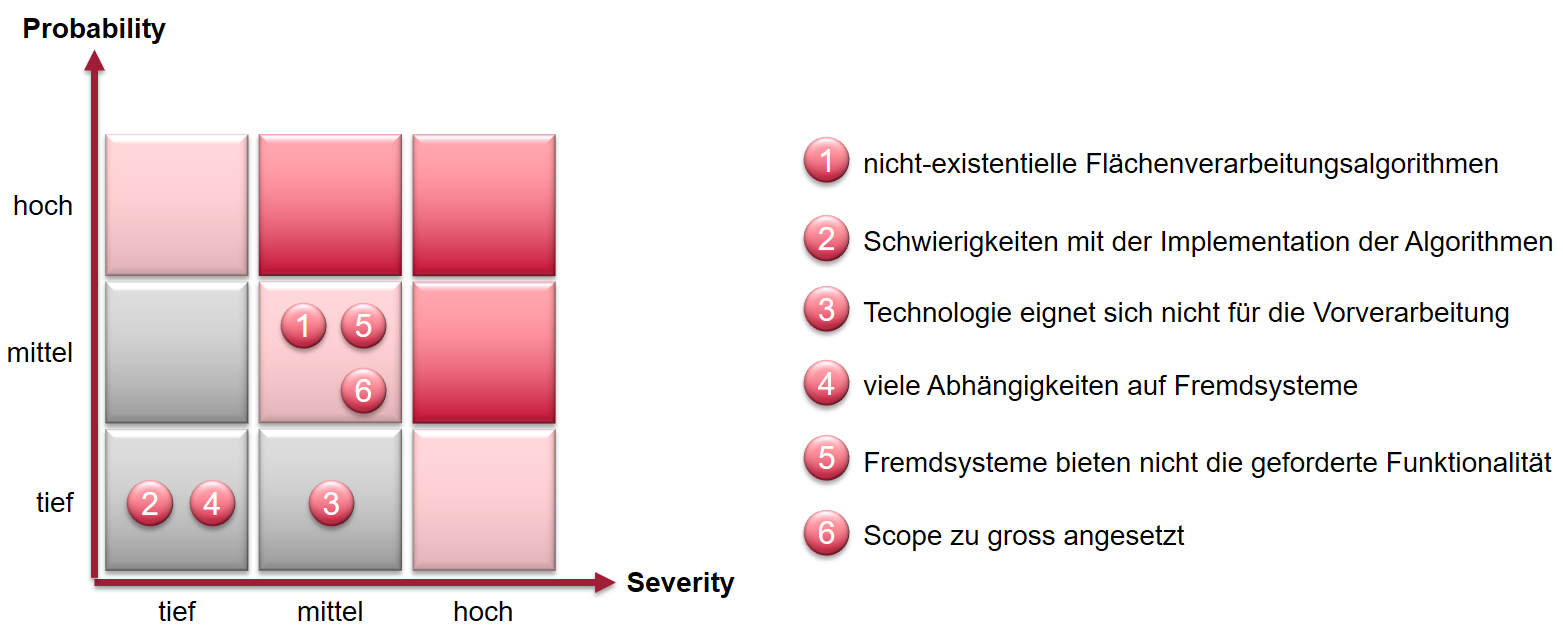
\includegraphics[width=1\linewidth]{projectdoc/img/risk_analysis}
    \caption[Risiko Analyse]{Risiko Analyse}
    \label{fig:risk_analysis}
\end{figure}

\subsubsection{Umgang mit Risiken}
\label{Risiken:Umang mit Risiken}
Um dem Hauptrisiko des Projekts, sprich die Evaluation, Optimierung und Implementation der Flächenverarbeitungsalgorithmen entgegen zu wirken, ist die erste Elaboration-Phase 4 Sprints lang und die Umsetzung der Algorithmen zu Beginn der Construction-Phase angesiedelt, um so genügend Spielraum zu haben. Treten in der ersten Elaboration-Phase Probleme mit diesem Punkt auf oder man sieht, dass sich Python für diesen Zweck nicht eignet, muss dementsprechend der Scope des Frontends (QGIS-Plugin) oder der zweite theoretische Teil gekürzt werden. Dies aus dem einfachen Grund, da ohne diese Grundlage auch keine Visualisierung und weitere theoretische Aufbereitung Sinn macht. Nach der Elaboration ist auch bekannt, ob alle Fremdsysteme die Anforderungen erfüllen. Ist dies nicht der Fall, können bei search.ch \cite{search_ch_route_api} Change-Requests beantragt werden. Je nach Priorisierung dieser durch search.ch muss der Zeitplan aktualisiert und der Scope gekürzt werden. Kann die Routing-Engine auf den vorverarbeitenden \ac{OSM}-Daten nicht operieren, so muss weiteren Aufwand in Anpassung der Verarbeitung der \ac{OSM}-Daten gesteckt werden, was ebenfalls eine Kürzung des Scopes zur Folge hat.

\subsubsection{Konsequenz}
\label{Risiken:Konsequenz}
Tritt eines der Hauptrisiken (WSK > 9) ein, muss der Prototyp (QGIS-Plugin) oder die zweite theoretische Aufarbeitung aus dem Scope gestrichen werden. Die kleineren Risiken vermindern die Funktionsweise des Prototyps.

\subsection{Team, Rollen und Verantwortlichkeiten}
\label{sub:Team, Rollen und Verantwortlichkeiten}

\begin{table}[H]
    \centering
    \caption{Team, Rollen und Verantwortlichkeiten}
    \label{table: Team, Rollen und Verantwortlichkeiten}
    \begin{tabular}{lll}
        & \textbf{Rolle} & \textbf{Verantwortlichkeiten}    \\
        Prof. Stefan Keller  &        Betreuer                   &    \\
        Robin Suter          &        Autor                      & Plaza Preprocessing \\
        Jonas Matter         &        Autor                      & PlazaRouting Backend, QGIS-Plugin
    \end{tabular}
\end{table}
\section{Projektmonitoring}
\label{sec:Projektmonitoring}

\subsection{Auswertung Velocity}
\label{sub:Auswertung Velocity}

\begin{figure}[H]
    \centering
    \begin{tikzpicture}
        \begin{axis}[
            ybar,
            width=1\textwidth,
            bar width=5pt,
            ylabel={Sprint Velocity},
            xlabel={Sprint Nr.},
            ymin=0,
            ymax=70,
            xtick=data,
            % nodes near coords,
            % nodes near coords align={vertical},
            % every node near coord/.append style={color=black, font=\tiny}
        ]
            \addplot[style={blue, fill=blue!30!white}] coordinates
                {(0, 29.5) (1, 46) (2, 45.5) (3, 46.5) (4, 44) (5, 35.5) (6, 35.5) (7, 35)
                (8, 32.5) (9, 34.5) (10, 47.5) (11, 55.5) (12, 55)};
            \addplot [style={red, fill=red!30!white}] coordinates
                {(0, 33.5) (1, 46) (2, 8.5) (3, 46.5) (4, 37) (5, 27.5) (6, 35.5) (7, 28)
                (8, 31.5) (9, 40.5) (10, 40) (11, 60.5) (12, 57)};
            \legend{Story-Points geplant,Story-Points erledigt}
        \end{axis}
    \end{tikzpicture}%

    \caption[Diagramm Sprint Velocity über das Projekt]{Sprint Velocity über den Verlauf des Projekts}
    \label{chart:sprint_velocity}
\end{figure}

In Abbildung \ref{chart:sprint_velocity} ist die Team Velocity für jeden Sprint über den Verlaufs des Projekts aufgezeichnet. Die Velocity besteht jeweils aus der Anzahl der geplanten und effektiv durchgeführten Story-Points. Jeder Sprint dauerte eine Woche.

Im Diagramm \ref{chart:sprint_velocity} ist auffällig, dass wir zu Beginn gerade eine hohe Velocity erreichten, die in Sprint 2 dann völlig einbrach. Dies lag hauptsächlich an zu grossen Arbeitspaketen, die kaum in einem Sprint erledigt werden konnten. Mit dieser Erkenntnis haben wir die weiteren Arbeitspakete aufgeteilt und im Sprint 3 wieder mit der Velocity von Sprint 2 geplant. Dies hat auch funktioniert, gegen Mitte des Projektes sinkte sie allerdings wieder auf ca. 35 und pendelte sich dort ein. Durch den Zeitdruck gegen Ende des Projektes stieg die Velocity wieder, damit wir die offenen Arbeitspakete noch vor dem Abgabetermin erledigen konnten.


\subsection{Zeitauswertung}
\label{sub:Zeitauswertung}

\begin{figure}[H]
    \centering
    \begin{tikzpicture}
        \begin{axis}[
            ybar,
            width=1\textwidth,
            bar width=10pt,
            ylabel={Geleistete Arbeitsstunden},
            xlabel={Woche},
            ymin=0,
            ymax=70,
            xtick=data,
            nodes near coords,
            nodes near coords align={vertical},
            every node near coord/.append style={color=black, font=\small}
        ]
            \addplot[style={orange, fill=orange!30!white}] coordinates
                {(1, 22.5) (2, 47.8) (3, 33) (4, 58.5) (5, 42) (6, 39.4) (7, 58.5)
                (8, 55.7) (9, 57) (10, 48.6) (11, 51.5) (12, 47.9) (13, 52) (14, 18.5)};
        \end{axis}
    \end{tikzpicture}

    \caption[Diagramm Zeitaufwand über den Verlauf des Projekts]{Zeitaufwand über den Verlauf des Projekts (Stand 19.12.2017)}
    \label{chart:Zeitauswertung}
\end{figure}

In Abbildung \ref{chart:Zeitauswertung} ist gezeigt, wie viele Stunden pro Woche über den Verlaufs des Projekts geleistet wurden. Das gesamte Zeitbudget betrug dabei \textbf{480} Stunden, was pro Woche ca. 34 Stunden entspricht.

Die total geleisteten Arbeitsstunden im Team sind mit \textbf{328h} (Jonas Matter) und \textbf{310h} (Robin Suter) ähnlich verteilt (Stand 19.12.2017).

Wie man in Abbildung \ref{chart:Zeitauswertung} sieht, ist die geleistete Zeit pro Woche ausser zu Beginn jeweils über dem eingeplanten Zeitbudget. Dies liegt wohl daran, dass wir um die Woche 4 eine hohe Velocity erreichten (siehe \ref{sub:Auswertung Velocity}), dafür aber viel Zeit investierten. In den nachfolgenden Wochen behielten wir die Velocity ungefähr bei, der Zeitaufwand blieb aber gleich hoch. Schlussendlich führte dies dazu, dass wir alle Projektziele erreichen konnten, dafür aber deutlich mehr Arbeitsaufwand als geplant investiert haben.

\subsection{Codestatistik}
\label{sub:Codestatistik}

In Tabelle \ref{table:Code-Metriken} sind einige Code-Metriken aufgelistet. Diese sind natürlich mit Vorsicht zu geniessen, da diese nur bedingt etwas über die Softwarequalität aussagen können. Es ist aber gut zu sehen, welchen Umfang die einzelnen Komponenten im Verhältnis zum Gesamtsystem ausmachen.

\begin{table}[ht]
    \centering
    \caption{Code-Metriken}
    \label{table:Code-Metriken}
    \begin{tabular}{p{10cm}r}
        \toprule
        \textbf{Anzahl Zeilen Produktiv-Code}           & \textbf{2328} \\
            \hspace{1em} \code{plaza\_preprocessing}    & 969           \\
            \hspace{1em} \code{plaza\_routing}          & 723           \\
            \hspace{1em} QGIS-Plugin                    & 636           \\
        \midrule
        \textbf{Anzahl Tests}                           & \textbf{74}   \\
            \hspace{1em} \code{plaza\_preprocessing}    & 29            \\
            \hspace{1em} \code{plaza\_routing}          & 45            \\
        \midrule
        \textbf{Test Coverage}                          & \textbf{83\%}   \\
            \hspace{1em} \code{plaza\_preprocessing}    & 88\%          \\
            \hspace{1em} \code{plaza\_routing}          & 78\%          \\
    \end{tabular}
\end{table}


\glsaddall
\printglossary[type=main,title=Glossar]


% \ac prints the longform the first time, after that the short
% using \acs always prints the shortform
   
\chapter*{Glossar und Abkürzungsverzeichnis}\addcontentsline{toc}{chapter}{Glossar und Abkürzungsverzeichnis}
\begin{acronym}[SFINAE] % [] should contain the longest acronym
    \acro{OSM}{Open Street Map}
    \acro{RUP}{Rational Unified Process}
\end{acronym}


\nocite{*}
\cleardoublepage % https://tex.stackexchange.com/a/98995
\phantomsection
\addcontentsline{toc}{chapter}{Literaturverzeichnis}
\bibliographystyle{IEEEtran}
\bibliography{PlazaRoute}

\cleardoublepage
\phantomsection
\addcontentsline{toc}{chapter}{Abbildungsverzeichnis}
\listoffigures

\cleardoublepage
\phantomsection
\addcontentsline{toc}{chapter}{Tabellenverzeichnis}
\listoftables

\renewcommand\listoflistingscaption{Code Listings}
\listoflistings
\addcontentsline{toc}{chapter}{Code Listings}

\end{document}
